\documentclass[12pt,a4paper]{report}

% Codificación y lenguaje
\usepackage[utf8]{inputenc}
\usepackage[T1]{fontenc}
\usepackage[spanish]{babel}
\decimalpoint

% Paquetes de citas y referencias
\usepackage[numbers,sort&compress]{natbib} % Para citas tipo [1-3] en lugar de [1],[2],[3]
\usepackage{hyperref}

% Paquetes matemáticos y de formato
\usepackage{amsmath,amssymb,amsfonts}
\usepackage{graphicx}
\graphicspath{{figuras/}} % Permite buscar imágenes en la carpeta raíz "figuras/"
\usepackage{geometry}
\usepackage{booktabs}
\usepackage{hyperref}
\usepackage{float}
\usepackage{setspace}
\usepackage{titlesec}
\usepackage{caption}

% Configuración de Márgenes para Trabajo de Grado / Tesis
\geometry{top=2.5cm, bottom=2.5cm, left=3.0cm, right=2.5cm}

% Interlineado 1.5 para lectura académica
\onehalfspacing

% Configuración de hipervínculos
\hypersetup{
    colorlinks=true,
    linkcolor=blue,
    citecolor=blue,
    urlcolor=blue,
    pdftitle={Simulación Dinámica y Diseño de un Acelerador Lineal tipo Álvarez},
    pdfauthor={Erick Mateo García Díaz}
}

% Formato de títulos de capítulos
\usepackage{titlesec}

% Formato compacto para Capítulos (Reducción de \Huge a \Large y menor espacio vertical)
\titleformat{\chapter}[display]
  {\normalfont\Large\bfseries\centering}
  {\chaptertitlename\ \thechapter}
  {6pt}
  {\large\bfseries}

% Ajuste de espacios verticales antes y después de cada capítulo
% \titlespacing*{comando}{izquierda}{espacio_arriba}{espacio_abajo}
\titlespacing*{\chapter}{0pt}{-10pt}{15pt}

% Reducción proporcional para Secciones y Subsecciones
\titleformat{\section}
  {\normalfont\large\bfseries}{\thesection}{1em}{}
\titlespacing*{\section}{0pt}{9pt}{6pt}

\titleformat{\subsection}
  {\normalfont\normalsize\bfseries}{\thesubsection}{1em}{}
\titlespacing*{\subsection}{0pt}{8pt}{4pt}

\begin{document}

% ==============================================================================
% PORTADA INSTITUCIONAL (UNIVERSIDAD DE NARIÑO)
% ==============================================================================
\begin{titlepage}
    \centering
    \vspace*{0.5cm}
    {\bfseries\Large UNIVERSIDAD DE NARIÑO \par}
    \vspace{0.3cm}
    {\bfseries\large FACULTAD DE CIENCIAS EXACTAS Y NATURALES \par}
    \vspace{0.2cm}
    {\bfseries\large DEPARTAMENTO DE FÍSICA \par}
    \vspace{1.8cm}
    
    {\huge\bfseries Simulación Dinámica y Diseño de un Acelerador Lineal (LINAC tipo Álvarez) \par}
    \vspace{0.5cm}
    {\large Trabajo de Investigación y Modelado Computacional \par}
    \vspace{2.0cm}
    
    {\large\textbf{Autores:}\par}
    {\large Erick Mateo García Díaz \par}
    \vspace{1.2cm}
    
    {\large\textbf{Asignatura:}\par}
    {Física Computacional 2 \par}
    \vspace{2.0cm}
    
    {\large San Juan de Pasto, Colombia \par}
    {\large \today \par}
\end{titlepage}


% ==============================================================================
% PÁGINAS PRELIMINARES
% ==============================================================================
\pagenumbering{roman}

\include{Resumen}
\include{Introduccion}

\newpage
\tableofcontents
\newpage
\listoffigures
\newpage
\listoftables
\newpage

\pagenumbering{arabic}


% ==============================================================================
% CAPÍTULO 1: INTRODUCCIÓN Y MARCO TEÓRICO
% ==============================================================================
\chapter{Marco Teórico}


\section{Planteamiento del Problema y Justificación}
El diseño de un LINAC tipo Álvarez requiere garantizar tres condiciones físicas simultáneas:
1. **Sincronismo Geométrico:** La longitud de cada celda debe coincidir exactamente con la distancia recorrida por la partícula síncrona en un período de la onda de RF ($L_n = \beta_n \lambda$).
2. **Estabilidad Longitudinal de Fase:** Las partículas desfasadas respecto al centro de masa del paquete deben experimentar una fuerza restauradora que limite el crecimiento de la emiteza longitudinal.
3. **Tolerancia Operativa de RF:** El acelerador debe ser tolerante a pequeñas desviaciones térmicas y de frecuencia en la fuente de potencia de RF sin perder la captura del haz.

Este trabajo desarrolla un simulador discreto en Python que resuelve las ecuaciones de transporte relativista celda a celda, generando un marco riguroso para analizar la emiteza, la tasa de aceleración espacial y las ventanas de tolerancia operacional del acelerador.
\section{Fundamentos Físicos y Formulación Matemática}

\subsection{Cinemática Relativista de Partículas Cargadas}
Para un protón con energía en reposo $m_0 c^2 = 938.272\text{ MeV}$, la energía cinética $T_n$ en la celda $n$ determina el factor de Lorentz $\gamma_n$ y la velocidad adimensional $\beta_n$:
\begin{equation}
\gamma_n = 1 + \frac{T_n}{m_0 c^2}
\end{equation}
\begin{equation}
\beta_n = \sqrt{1 - \frac{1}{\gamma_n^2}} = \frac{\sqrt{T_n (T_n + 2 m_0 c^2)}}{T_n + m_0 c^2}
\end{equation}

\subsection{Condición de Sincronismo y Longitud de Celda}
En una cavidad resonante que oscila a frecuencia angular $\omega = 2\pi f_{\text{RF}}$ con longitud de onda en el vacío $\lambda = c / f_{\text{RF}}$, el tiempo transcurrido mientras la partícula cruza una celda de longitud $L_n$ debe ser exactamente igual a un período de RF ($\tau = 1/f_{\text{RF}}$):
\begin{equation}
\Delta t_n = \frac{L_n}{\beta_n c} = \frac{1}{f_{\text{RF}}} \implies L_n = \beta_n \lambda
\end{equation}

\subsection{Ganancia de Energía y Estabilidad de Fase}
La ganancia de energía cinética de la partícula síncrona al atravesar el hueco de aceleración (\textit{gap}) de la celda $n$ está dada por:
\begin{equation}
\Delta T_n = q V_{\text{gap}} \cos(\phi_s)
\end{equation}
donde $V_{\text{gap}} = 1.0\text{ MV}$ es la tensión de pico y $\phi_s = -30^\circ$ es la fase síncrona. La elección de $\phi_s < 0$ garantiza la estabilidad del pozo de potencial síncrono. Una partícula con una desviación de fase $\Delta\phi_i = \phi_i - \phi_s$ experimenta una fuerza restauradora dada por la ecuación diferencial de oscilación longitudinal:
\begin{equation}
\frac{d}{dn} \left( m_0 c^2 \beta_n^3 \gamma_n^3 \frac{d(\Delta\phi)}{dn} \right) + 2\pi q V_{\text{gap}} \sin(\phi_s) \Delta\phi = 0
\end{equation}

\subsection{Definición de Campos Eléctricos y Atenuación Geométrica}
Definimos el gradiente medio pico por celda $E_{0,n}$ y el gradiente de aceleración síncrono efectivo $E_{\text{acc},n}$ como:
\begin{equation}
E_{0,n} = \frac{q V_{\text{gap}}}{L_n}, \quad E_{\text{acc},n} = \frac{\Delta T_n}{L_n} = E_{0,n} \cos(\phi_s)
\end{equation}
A medida que $\beta_n$ aumenta y las celdas se expanden en la dirección longitudinal $z$, el campo efectivo por unidad de longitud decae de forma inversamente proporcional a $L_n$.

% ==============================================================================
% CAPÍTULO 2: METODOLOGÍA COMPUTACIONAL Y ARQUITECTURA DEL SIMULADOR
% ==============================================================================
\chapter{Metodología Computacional y Arquitectura del Simulador}

\section{Arquitectura del Software y Estructura Modular}
El simulador dinámico fue desarrollado en Python 3 siguiendo una arquitectura modular orientada a separar la física fundamental, el cálculo geométrico, la integración discreta de trayectorias, el análisis de estabilidad y la visualización analítica. El código fuente reside en el directorio \texttt{src/} y se estructura en los siguientes módulos:

\begin{description}
    \item[\texttt{physics.py}:] Contiene las constantes físicas fundamentales ($c$, $m_0 c^2_{\text{proton}}$, $m_0 c^2_{\text{electron}}$, $q$) y las funciones de conversión cinemática para calcular el factor de Lorentz $\gamma$ y la velocidad adimensional $\beta$.
    \item[\texttt{linac\_design.py}:] Implementa el diseño síncrono geométrico celda a celda, resolviendo la longitud $L_n = \beta_n \lambda$, la posición acumulada $z_n$, la ganancia energética $\Delta T_n = q V_{\text{gap}} \cos(\phi_s)$ y los campos eléctricos $E_{0,n}$ y $E_{\text{acc},n}$. Exporta los datos a \texttt{resultados/diseno\_celdas.csv}.
    \item[\texttt{tracking.py}:] Genera el paquete inicial de $N = 3000$ protones con dispersiones gaussianas y ejecuta el algoritmo de transporte numérico discreto en el plano de fases $(\Delta\phi, \Delta T)$ a través de las 55 celdas.
    \item[\texttt{synchrotron.py}:] Simula las oscilaciones de sincrotrón no lineales para perturbaciones discretas de fase, comparando el avance de fase numérico frente al valor teórico de oscilación de fase $\mu_n$.
    \item[\texttt{rf\_errors.py}:] Modula la frecuencia angular de RF ($\omega = \omega_0 (1 + \epsilon_f)$) para evaluar la sensibilidad del haz y el desplazamiento del punto síncrono ante errores del $0\%$ al $4\%$.
    \item[\texttt{electrons.py}:] Modela el comportamiento de un haz ultrarelativista de electrones ($T_0 = 10.0\text{ MeV}$) en una cavidad de celdas constantes de longitud $L = \lambda$.
    \item[\texttt{visualizer.py}:] Centraliza las rutinas de generación gráfica produciendo 11 figuras analíticas con resolución de 300 DPI almacenadas en el directorio \texttt{figuras/}.
    \item[\texttt{main.py}:] Script principal de orquestación que ejecuta secuencialmente todas las etapas del simulador y actualiza los archivos CSV y las imágenes.
\end{description}

\section{Algoritmo de Integración Discreta Celda a Celda}
El transporte del haz a través de la cavidad tipo Álvarez se modela mediante un esquema de integración paso a paso celda por celda. Para una partícula $i$ en la celda $n$, la actualización de su energía cinética y su fase de RF se rige por el par de ecuaciones discretas:

\begin{equation}
T_{i, n+1} = T_{i, n} + q V_{\text{gap}} \cos(\phi_{i, n})
\end{equation}

\begin{equation}
\phi_{i, n+1} = \phi_{i, n} + 2\pi \left( \frac{L_n \cdot f_{\text{RF}}}{\beta_{i, n+1} c} - 1 \right)
\end{equation}

donde $\beta_{i, n+1}$ se recalcula dinámicamente tras la ganancia de energía en el hueco mediante:
\begin{equation}
\beta_{i, n+1} = \sqrt{1 - \left( 1 + \frac{T_{i, n+1}}{m_0 c^2} \right)^{-2}}
\end{equation}

Este esquema conserva la estructura simpléctica del espacio de fases en el régimen de oscilaciones pequeñas y permite registrar con alta precisión la trayectoria de cada partícula del paquete.

\section{Generación del Paquete de Partículas y Espacio de Fases Inicial}
Para simular un haz realista, se genera una población de $N = 3000$ protones utilizando distribuciones gaussianas independientes en energía y fase alrededor de la partícula síncrona nominal ($T_0 = 3.0\text{ MeV}$, $\phi_s = -30^\circ$):

\begin{equation}
T_{i, 0} \sim \mathcal{N}\left(T_0, \sigma_T^2\right), \quad \text{con } \sigma_T = 0.005 \cdot T_0 = 15.0\text{ keV}
\end{equation}
\begin{equation}
\phi_{i, 0} \sim \mathcal{N}\left(\phi_s, \sigma_\phi^2\right), \quad \text{con } \sigma_\phi = 15.0^\circ
\end{equation}

Se define como criterio de aceptación o captura longitudinal que la partícula finalice el recorrido en la celda 55 permaneciendo dentro de una ventana de fase de $|\phi_{i, 55} - \phi_s| < 60^\circ$.

\section{Metodología de Exportación de Datos y Visualizaciones Analíticas}
El simulador garantiza la reproducibilidad científica mediante la exportación automatizada de datasets en formato CSV dentro del directorio \texttt{resultados/} utilizando la librería \texttt{pandas}. Asimismo, el módulo \texttt{visualizer.py} genera gráficos vectoriales y matriciales procesados a 300 DPI en \texttt{figuras/}, asegurando la independencia del entorno de ejecución ya sea desde la terminal (\texttt{main.py}) o mediante el cuaderno interactivo \texttt{P19-Acelerador-lineal.ipynb}.
% ==============================================================================
% CAPÍTULO 3: DISEÑO GEOMÉTRICO Y PERFILES DE CAMPO ELÉCTRICO
% ==============================================================================
\chapter{Diseño Geométrico y Perfiles de Campo Eléctrico}

\section{Evolución Geométrico-Cinemática de las Celdas Síncronas}
El diseño de la cavidad resonante tipo Álvarez para la aceleración de protones se fundamenta en la estricta preservación de la condición de sincronismo relativista celda a celda. Para una frecuencia de radiofrecuencia nominal $f_{\text{RF}} = 352.2\text{ MHz}$, la longitud de onda en el vacío del campo electromagnético es $\lambda = c / f_{\text{RF}} \approx 0.8512\text{ m}$.

Dado que la ganancia de energía cinética por celda para la partícula síncrona es constante ($\Delta T = q V_{\text{gap}} \cos\phi_s = 1.0\text{ MV} \cdot \cos(-30^\circ) \approx 0.866025\text{ MeV}$), la energía acumulada al finalizar la celda $n$ aumenta de forma estrictamente lineal de acuerdo con:
\begin{equation}
T_n = T_0 + n \cdot q V_{\text{gap}} \cos(\phi_s)
\end{equation}

Como consecuencia del incremento sostenido en la energía cinética de $T_0 = 3.0\text{ MeV}$ a $T_{55} = 50.631\text{ MeV}$, el factor relativista de velocidad $\beta_n$ pasa de $0.0905$ en la primera celda a $0.3159$ en la celda final. Por lo tanto, las celdas síncronas experimentan una expansión longitudinal continua calculada mediante $L_n = \beta_n \lambda$, pasando de $L_1 = 0.077033\text{ m}$ ($7.70\text{ cm}$) a $L_{55} = 0.268874\text{ m}$ ($26.89\text{ cm}$).

\begin{figure}[H]
    \centering
    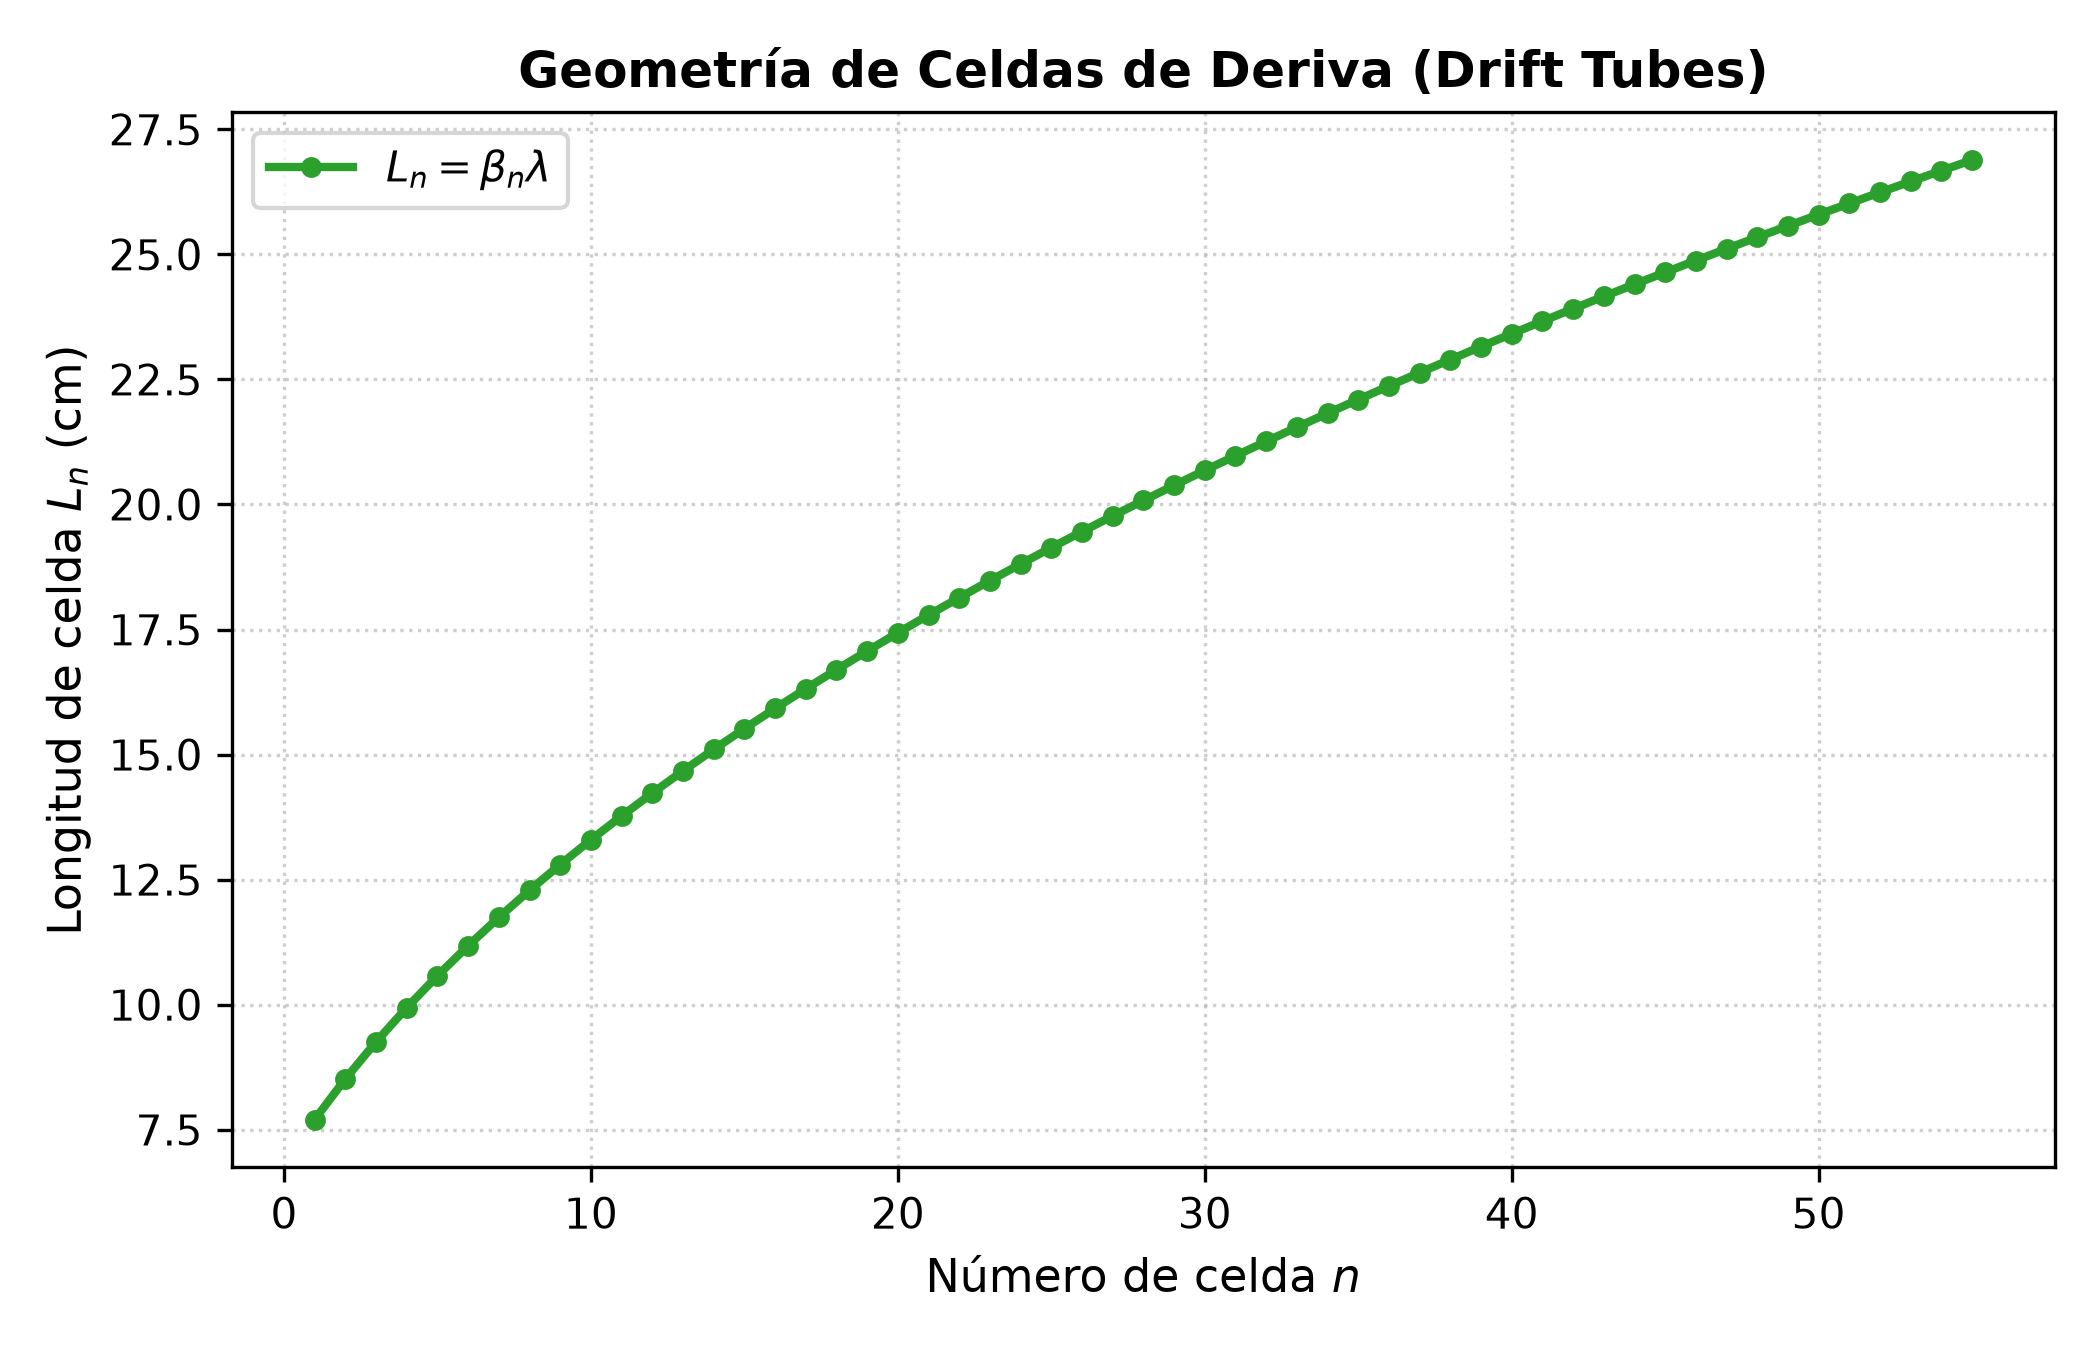
\includegraphics[width=0.85\textwidth]{figuras/fig01_diseno.png}
    \caption{Perfil geométrico del incremento de longitud de celdas síncronas $L_n = \beta_n \lambda$ a lo largo de las 55 celdas del LINAC Álvarez.}
    \label{fig:diseno_celdas}
\end{figure}

En la Figura \ref{fig:diseno_celdas} se aprecia la curvatura cóncava inicial en la longitud de las celdas, reflejando el rápido cambio cinemático en el régimen no relativista ($\beta \propto \sqrt{T}$ para $T \ll m_0 c^2$), seguida de una transición gradualmente lineal a medida que la inercia relativista limita la aceleración efectiva.

\section{Distribución del Campo Eléctrico y Gradientes de Aceleración}
Un aspecto físico central en el análisis de cavidades resonantes tipo Álvarez es la distinción formal entre el gradiente pico nominal $E_{0,n}$ y el gradiente de aceleración síncrono efectivo $E_{\text{acc},n}$. Ambas magnitudes se definen como promedios espaciales sobre la longitud total de la celda $n$:

\begin{equation}
E_{0,n} = \frac{q V_{\text{gap}}}{L_n} = \frac{1.0\text{ MV}}{L_n}
\end{equation}

\begin{equation}
E_{\text{acc},n} = \frac{\Delta T}{L_n} = \frac{q V_{\text{gap}} \cos(\phi_s)}{L_n} = E_{0,n} \cos(\phi_s)
\end{equation}

Dado que la tensión en el hueco de aceleración ($V_{\text{gap}} = 1.0\text{ MV}$) se mantiene constante a lo largo de toda la cavidad, la densidad de aceleración por unidad de longitud ($\text{MV/m}$) disminuye de forma inversamente proporcional a la longitud de la celda $L_n$.

\begin{figure}[H]
    \centering
    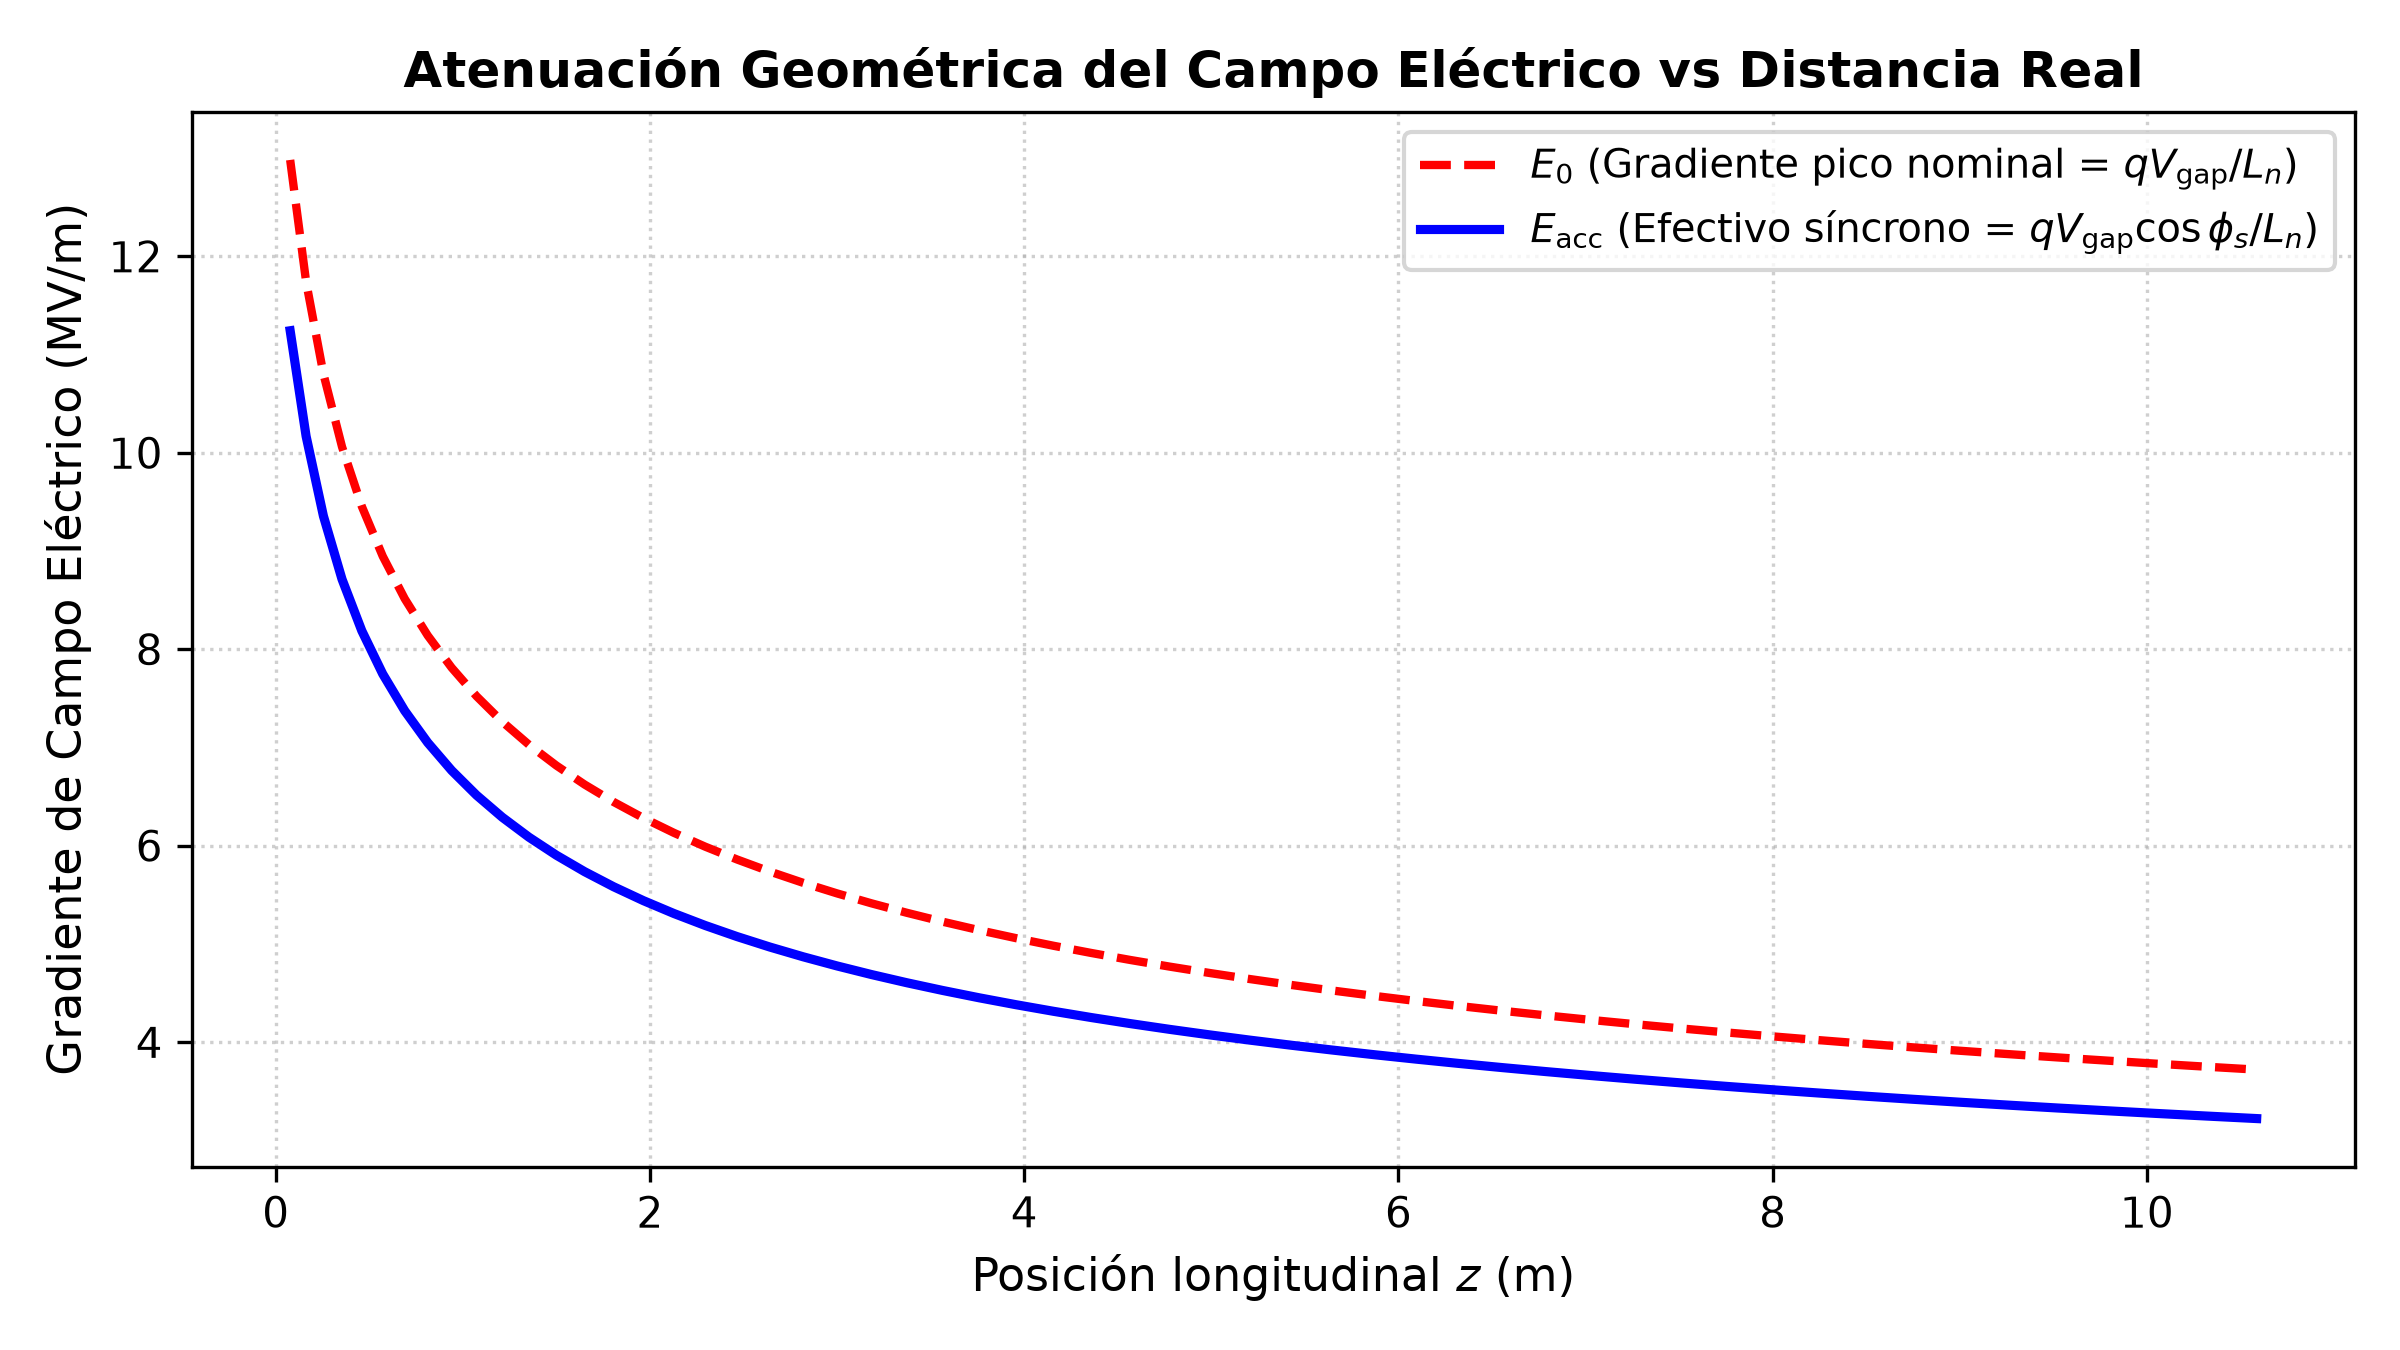
\includegraphics[width=0.88\textwidth]{figuras/fig06_perfil_campos.png}
    \caption{Perfil de atenuación geométrica del gradiente de campo eléctrico pico nominal ($E_0$) y del gradiente de aceleración efectivo síncrono ($E_{\text{acc}}$) en función de la posición longitudinal real $z$ (m).}
    \label{fig:perfil_campos}
\end{figure}

Como se ilustra en la Figura \ref{fig:perfil_campos}:
\begin{itemize}
    \item En la región de inyección ($z = 0.077\text{ m}$, Celda 1), el acelerador requiere un gradiente efectivo elevado de $E_{\text{acc},1} = 11.242\text{ MV/m}$ ($E_{0,1} = 12.981\text{ MV/m}$) debido a la brevedad del recorrido de la celda ($7.70\text{ cm}$).
    \item En la región de extracción ($z = 10.587\text{ m}$, Celda 55), la distribución de la misma ganancia energética ($0.866\text{ MeV}$) sobre una distancia mayor ($26.89\text{ cm}$) diluye el gradiente efectivo a $E_{\text{acc},55} = 3.221\text{ MV/m}$ ($E_{0,55} = 3.719\text{ MV/m}$).
\end{itemize}

\section{Perfil Cinemático Combinado y Resumen Geométrico}
La acumulación espacial de las longitudes de las 55 celdas determina una longitud total de la cavidad resonante de $z_{\text{total}} = 10.5867\text{ m} \approx 10.59\text{ m}$.

En la Figura \ref{fig:perfil_cinematico} se presenta la evolución simultánea de la velocidad relativa $\beta = v/c$ (eje izquierdo) y la energía cinética $T$ (eje derecho) respecto a la coordenada axial continua $z$.

\begin{figure}[H]
    \centering
    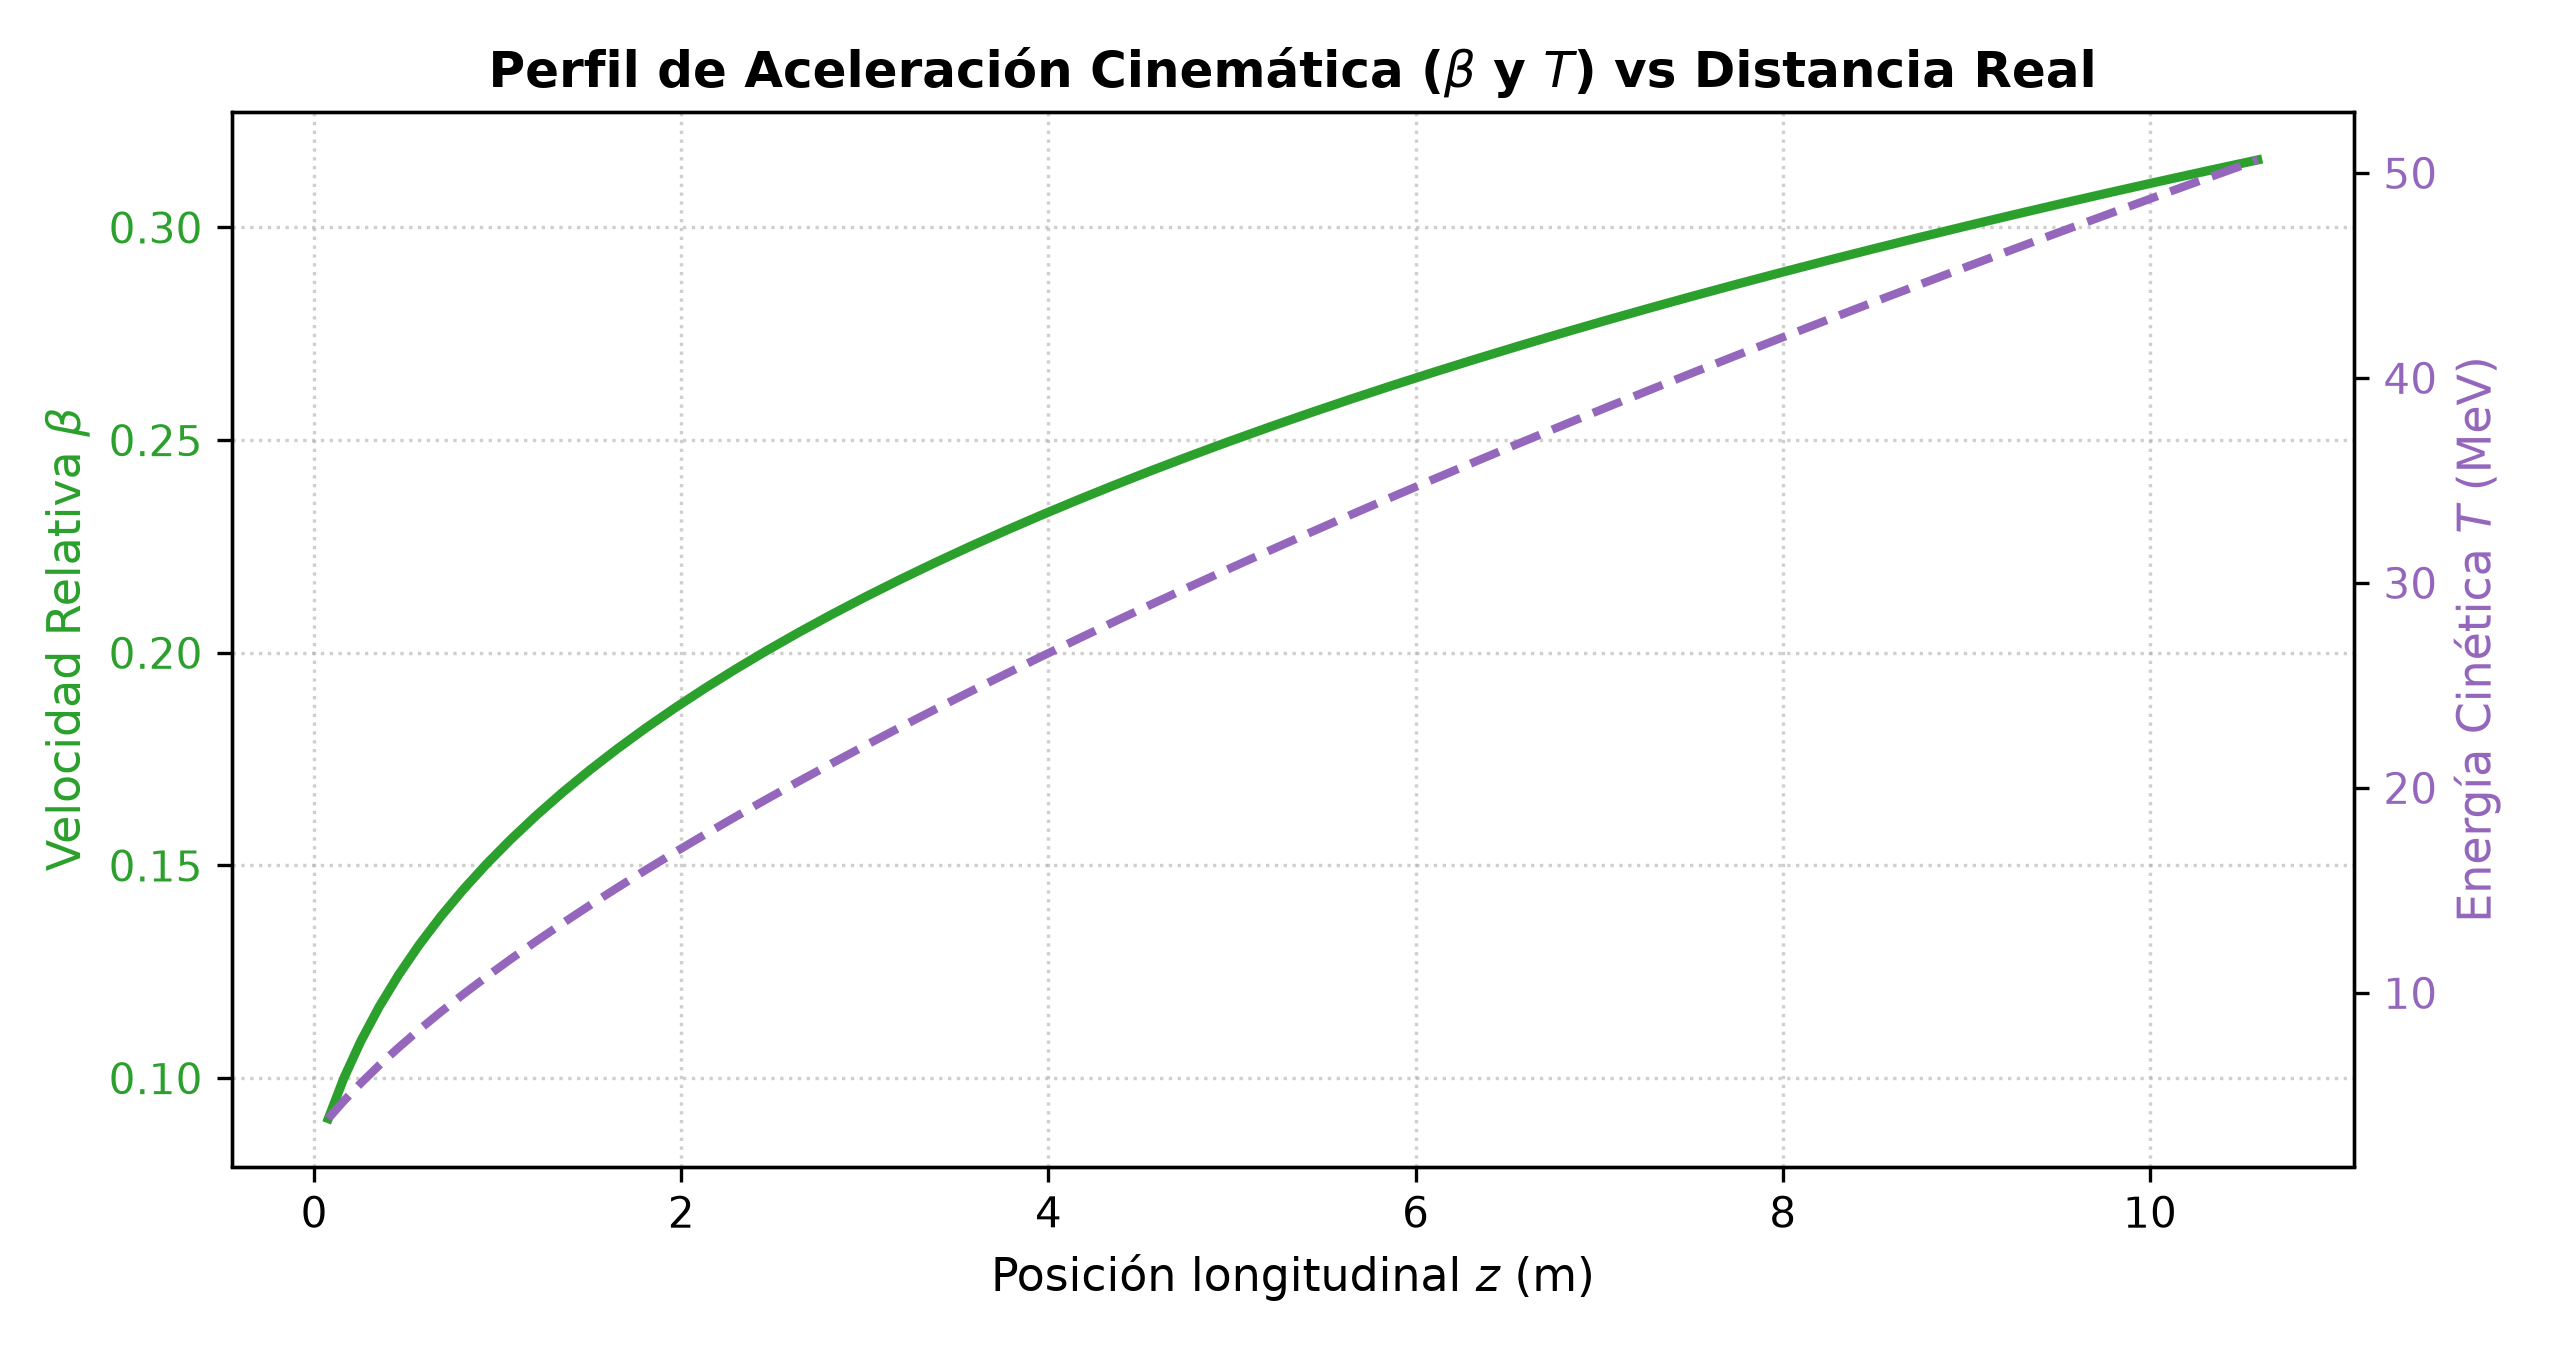
\includegraphics[width=0.88\textwidth]{figuras/fig08_perfil_cinematico.png}
    \caption{Perfil combinado de aceleración cinemática: evolución de la velocidad adimensional $\beta$ y la energía cinética síncrona $T$ (MeV) en función de la distancia longitudinal $z$.}
    \label{fig:perfil_cinematico}
\end{figure}

\begin{table}[H]
    \centering
    \caption{Parámetros cinemáticos, geométricos y de campo eléctrico para celdas representativas del LINAC Álvarez de 55 celdas.}
    \label{tab:diseno_resumen}
    \vspace{0.2cm}
    \small
    \setlength{\tabcolsep}{4pt}
    \resizebox{\textwidth}{!}{%
    \begin{tabular}{cccccccc}
        \toprule
        \textbf{Celda $n$} & $L_n$ (m) & $z_n$ (m) & $T_{\text{sync}}$ (MeV) & $\beta$ & $\gamma$ & $E_{\text{acc}}$ (MV/m) & $E_0$ (MV/m) \\
        \midrule
        1  & 0.077033 & 0.077033 & 3.866 & 0.0905 & 1.0041 & 11.242 & 12.981 \\
        10 & 0.132959 & 1.118991 & 11.660 & 0.1562 & 1.0124 & 6.513  & 7.521  \\
        20 & 0.174780 & 2.664402 & 20.321 & 0.2053 & 1.0217 & 4.955  & 5.721  \\
        30 & 0.207865 & 4.582845 & 28.981 & 0.2442 & 1.0309 & 4.166  & 4.811  \\
        40 & 0.235955 & 6.806297 & 37.641 & 0.2772 & 1.0401 & 3.670  & 4.238  \\
        50 & 0.260191 & 9.294488 & 46.301 & 0.3057 & 1.0493 & 3.328  & 3.843  \\
        55 & 0.268874 & 10.586696 & 50.631 & 0.3159 & 1.0540 & 3.221  & 3.719  \\
        \bottomrule
    \end{tabular}%
    }
\end{table}
% ==============================================================================
% CAPÍTULO 4: DINÁMICA MULTIPARTÍCULA Y ESPACIO DE FASES
% ==============================================================================
\chapter{Dinámica Multipartícula, Espacio de Fases y Amortiguamiento Adiabático}

\section{Evolución del Paquete de Partículas en el Espacio de Fases}
Para caracterizar la estabilidad longitudinal del haz, se realizó el seguimiento discreto de un paquete de $N = 3000$ protones a lo largo de las 55 celdas del LINAC Álvarez. Las partículas se inyectaron a $T_0 = 3.0\text{ MeV}$ con distribuciones gaussianas ($\sigma_T = 15.0\text{ keV}$, $\sigma_\phi = 15.0^\circ$) centradas en la fase síncrona $\phi_s = -30^\circ$.

\begin{figure}[H]
    \centering
    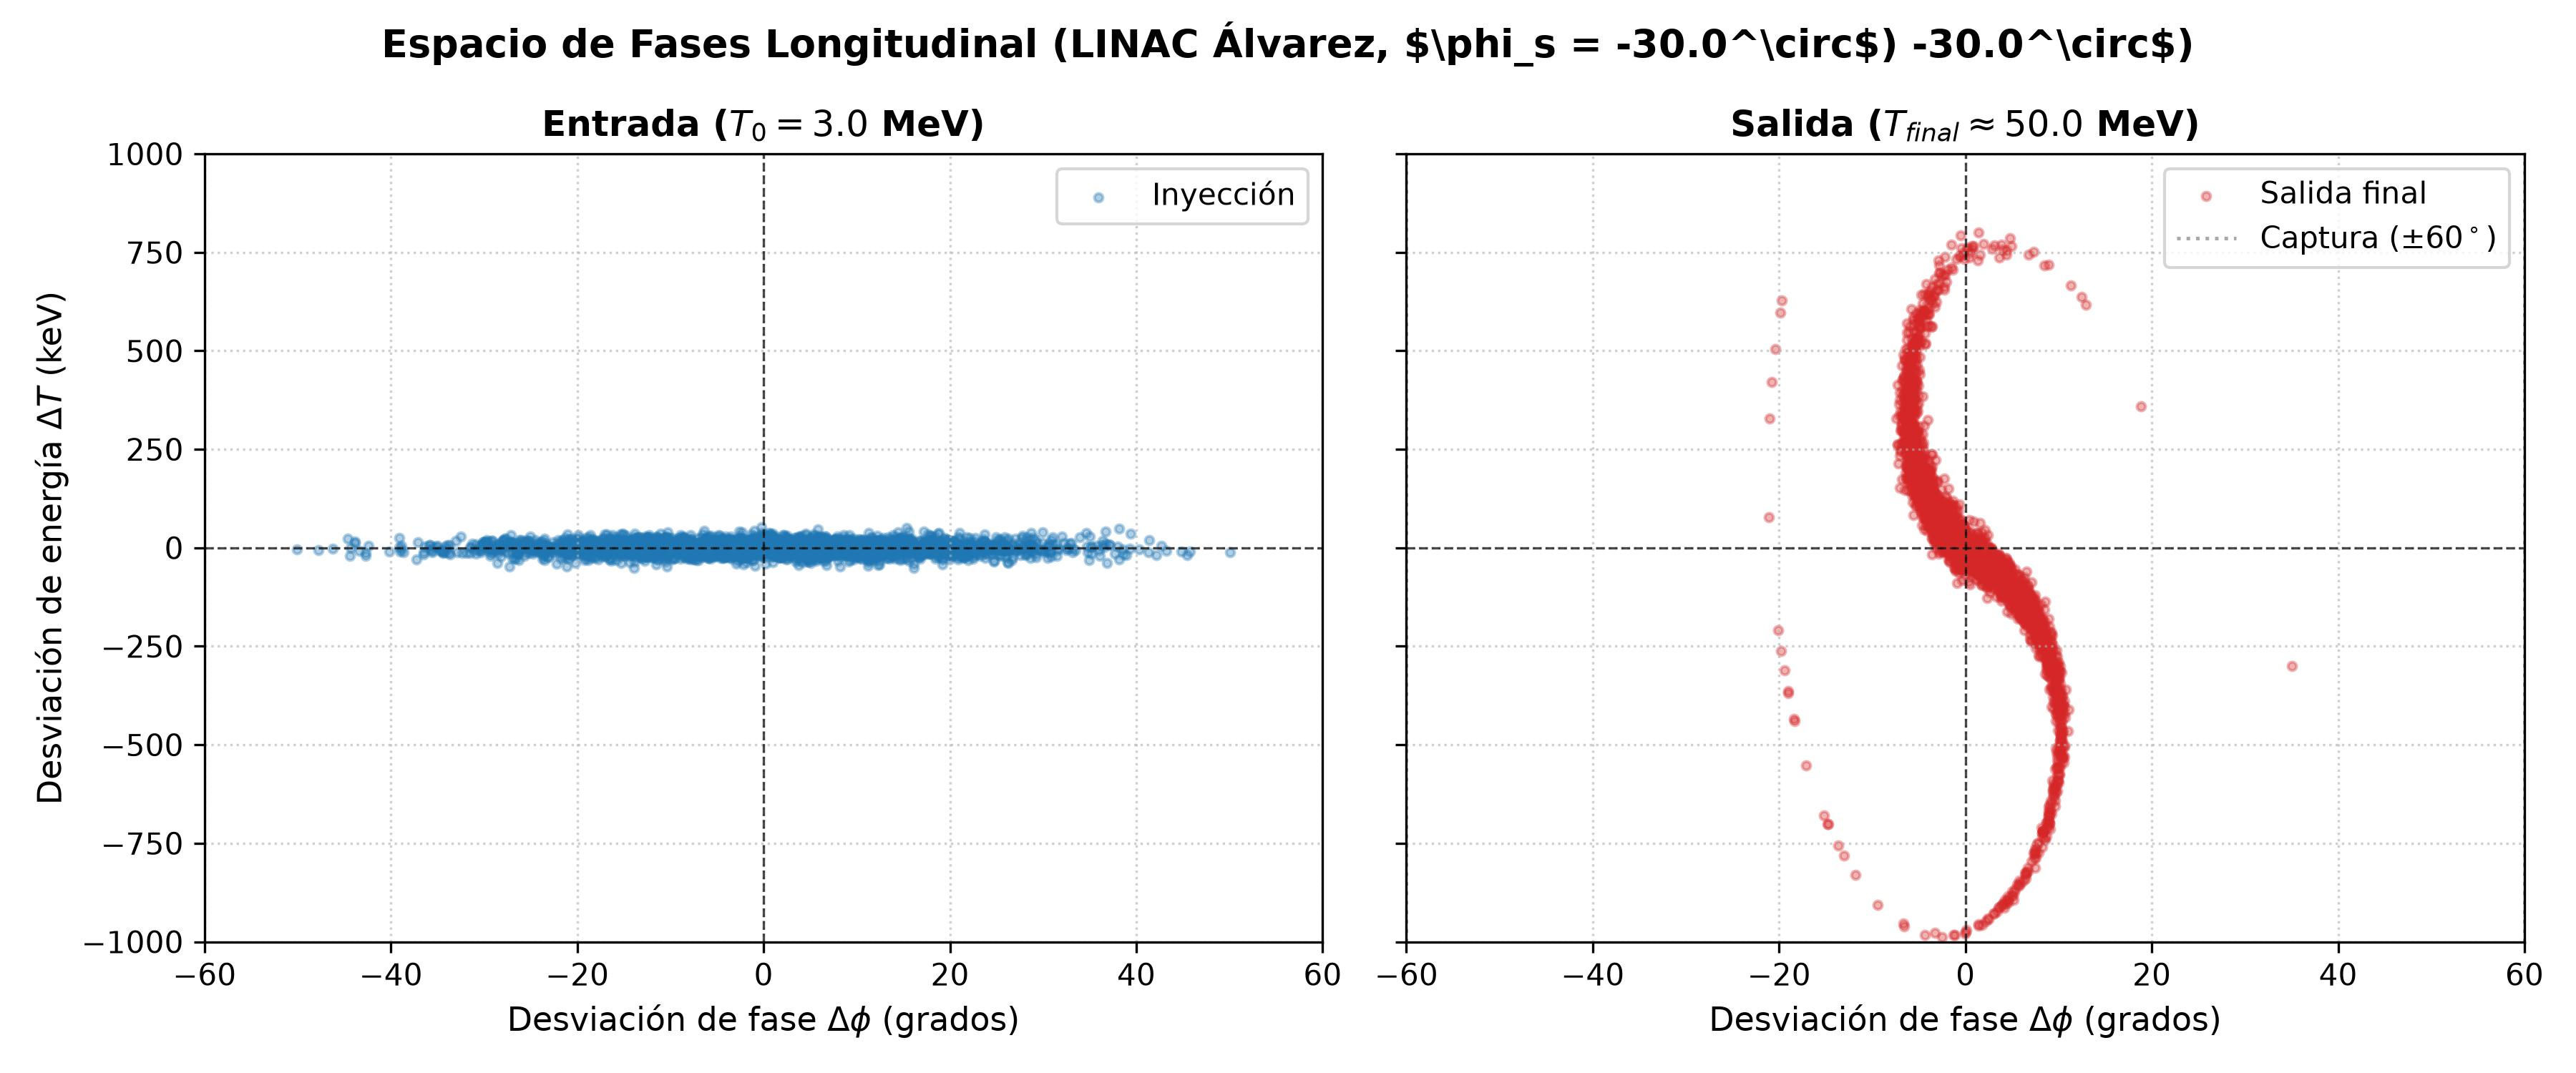
\includegraphics[width=0.88\textwidth]{figuras/fig02_espacio_fases.png}
    \caption{Rotación del haz de 3000 protones en el espacio de fases $(\Delta\phi, \Delta T)$ desde la inyección en Celda 1 (3.0 MeV) hasta la extracción en Celda 55 (50 MeV).}
    \label{fig:espacio_fases}
\end{figure}

Como se observa en la Figura \ref{fig:espacio_fases}, la distribución de partículas experimenta un movimiento de rotación coherente en el espacio de fases $(\Delta\phi, \Delta T)$ a medida que oscila alrededor del punto fijo síncrono. En la celda final (55), el $99.1\%$ de las partículas permanecen confinadas dentro de la región de estabilidad longitudinal.

\section{Demostración del Teorema de Liouville y Amortiguamiento Adiabático}
De acuerdo con el Teorema de Liouville, la emiteza longitudinal empaquetada debe mantenerse constante durante un proceso hamiltoniano sin pérdidas. Sin embargo, en coordenadas físicas $(\Delta\phi, \Delta T)$, el incremento sostenido del momento relativista del protón ($\beta\gamma$) produce el fenómeno de \textit{amortiguamiento adiabático}.

Las amplitudes de oscilación de la dispersión de fase ($\sigma_\phi$) y de la dispersión de energía ($\sigma_T$) evolucionan según las relaciones de proporcionalidad:
\begin{equation}
\sigma_\phi(n) \propto (\beta_n \gamma_n)^{-3/4}, \quad \sigma_T(n) \propto (\beta_n \gamma_n)^{3/4}
\end{equation}

\begin{figure}[H]
    \centering
    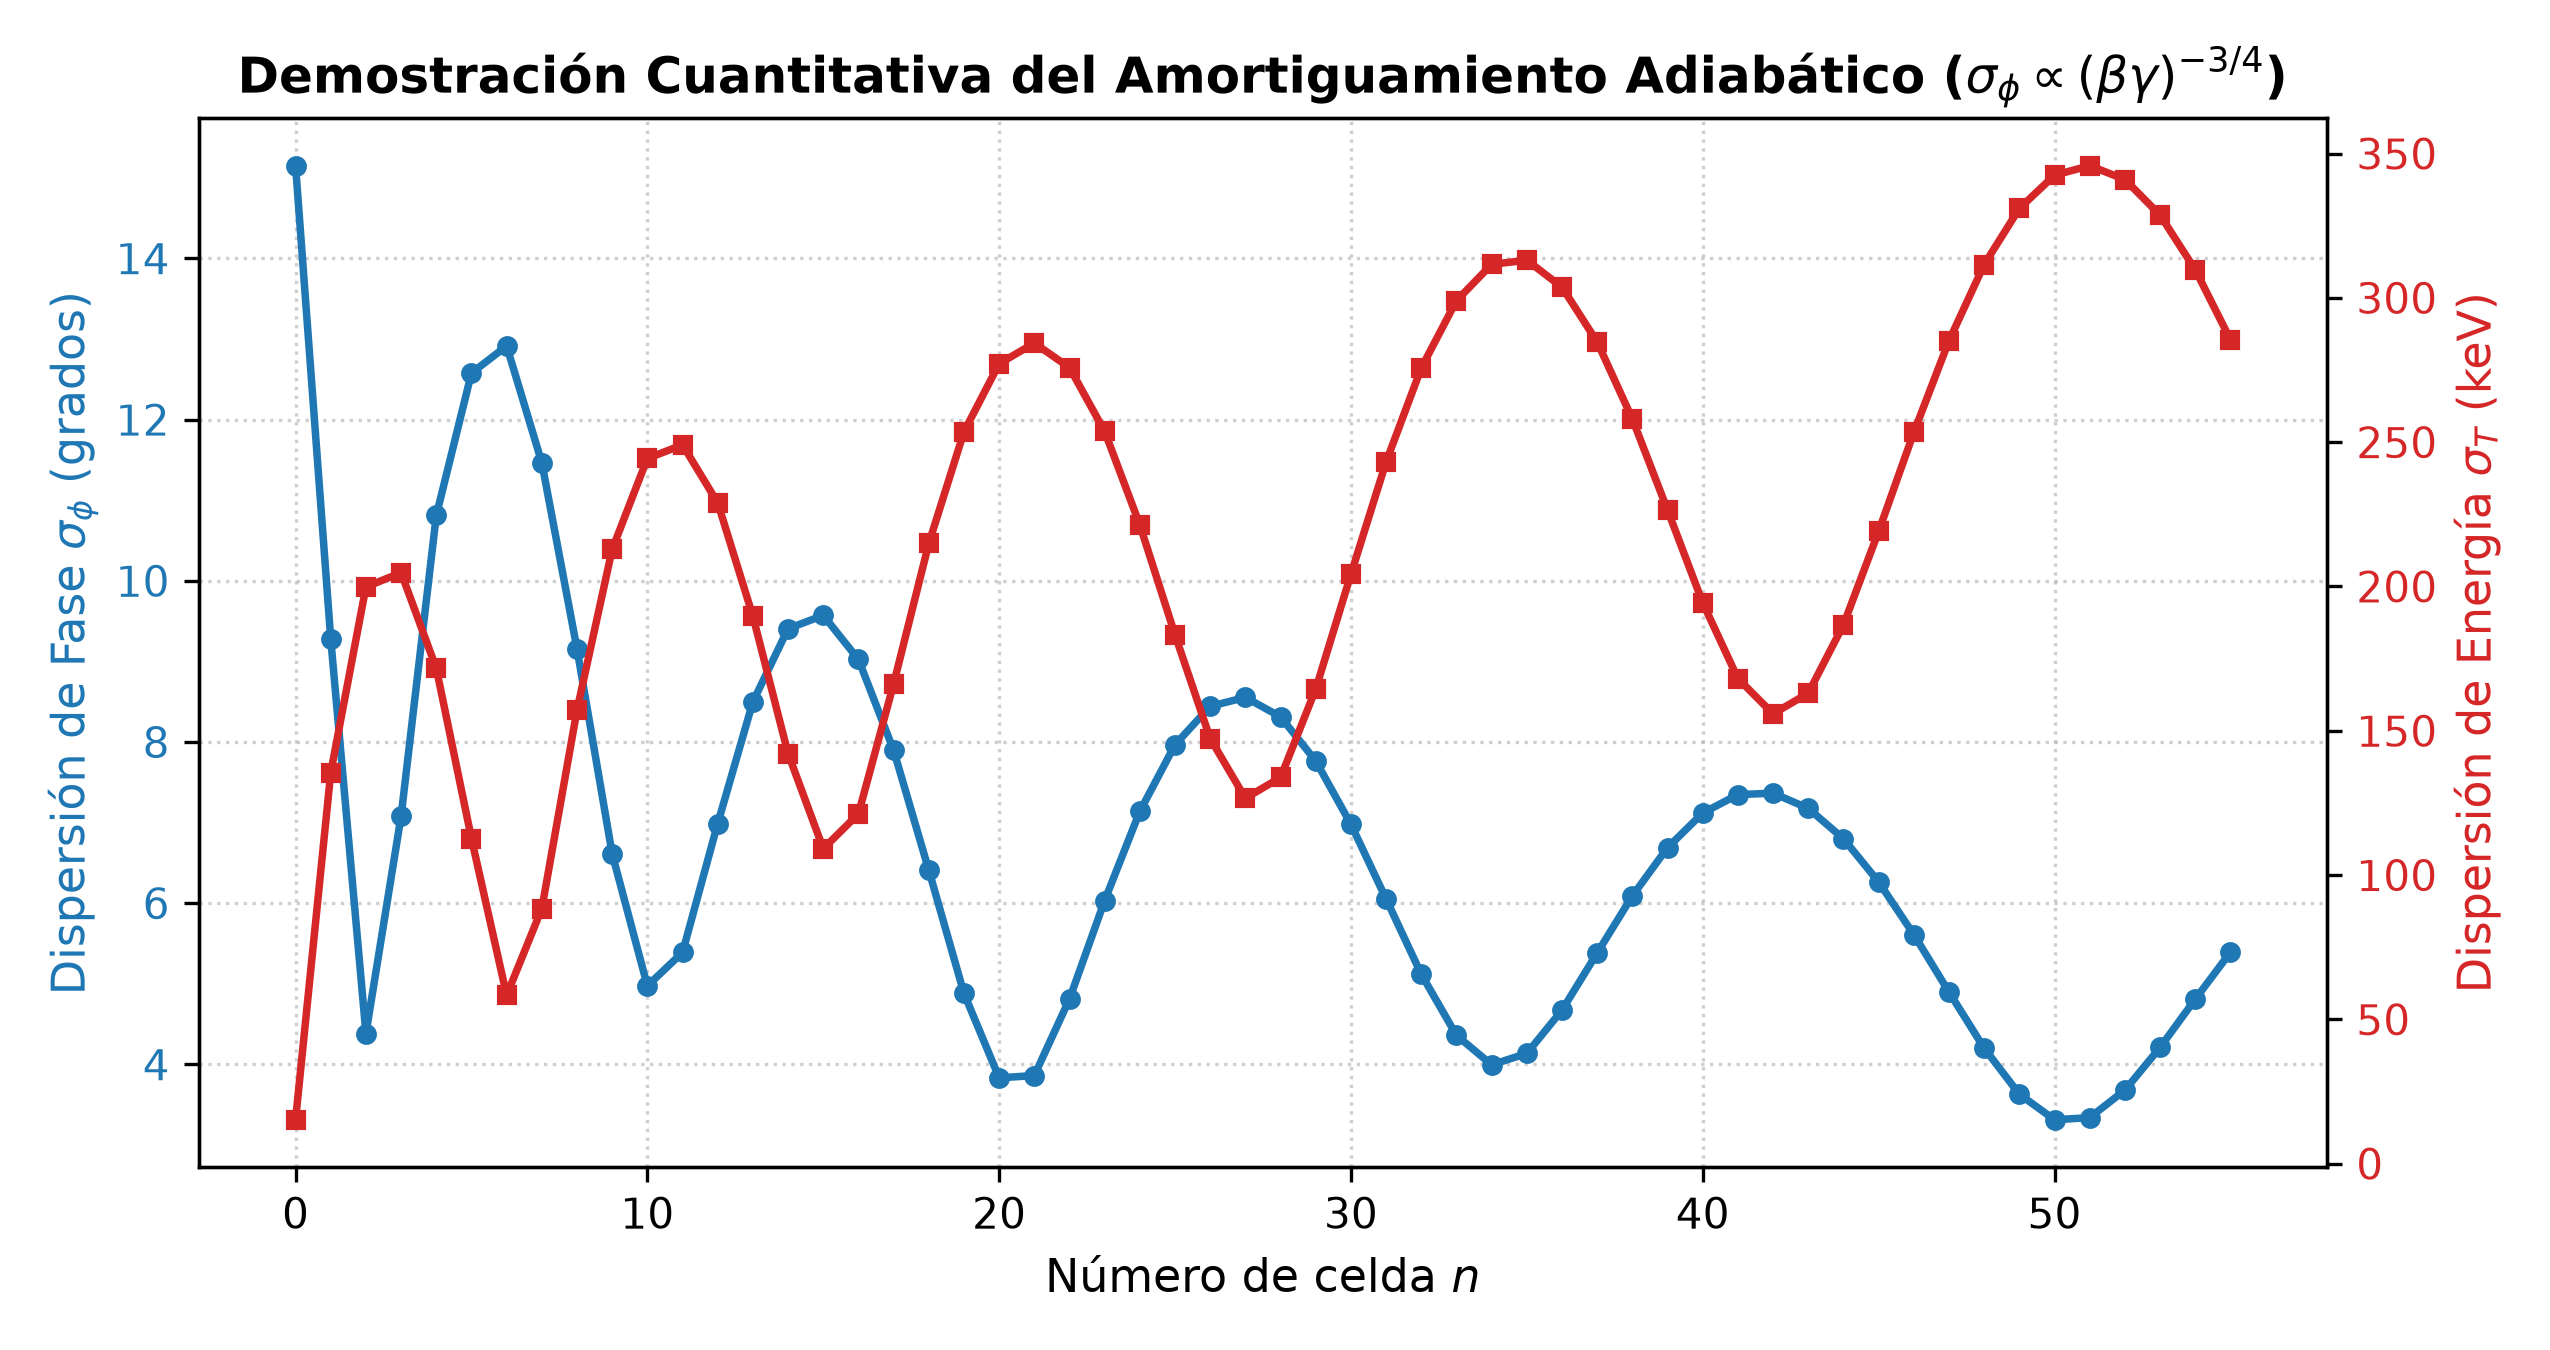
\includegraphics[width=0.88\textwidth]{figuras/fig07_amortiguamiento_cuantitativo.png}
    \caption{Evolución celda a celda del amortiguamiento adiabático: compresión de la dispersión de fase $\sigma_\phi$ (grados) frente a la expansión de la dispersión de energía $\sigma_T$ (keV).}
    \label{fig:amortiguamiento_cuantitativo}
\end{figure}

La Figura \ref{fig:amortiguamiento_cuantitativo} confirma cuantitativamente esta predicción teórica:
\begin{itemize}
    \item La dispersión estándar de fase $\sigma_\phi$ se comprime drásticamente desde $\sigma_{\phi, 0} = 15.19^\circ$ en la inyección hasta $\sigma_{\phi, 55} = 5.27^\circ$ en la extracción.
    \item La dispersión de energía $\sigma_T$ se expande desde $\sigma_{T, 0} = 15.15\text{ keV}$ hasta $\sigma_{T, 55} = 284.47\text{ keV}$, preservando el producto del área total en el espacio de fases.
\end{itemize}

\section{Mapa de Densidad 2D del Haz Extraído}
Para modelar las mediciones de los monitores de perfil longitudinal de intensidad de haz (*beam profile monitors*), en la Figura \ref{fig:densidad_emiteza} se presenta el mapa de densidad bidimensional (histograma 2D de frecuencia) del paquete en la Celda 55.

\begin{figure}[H]
    \centering
    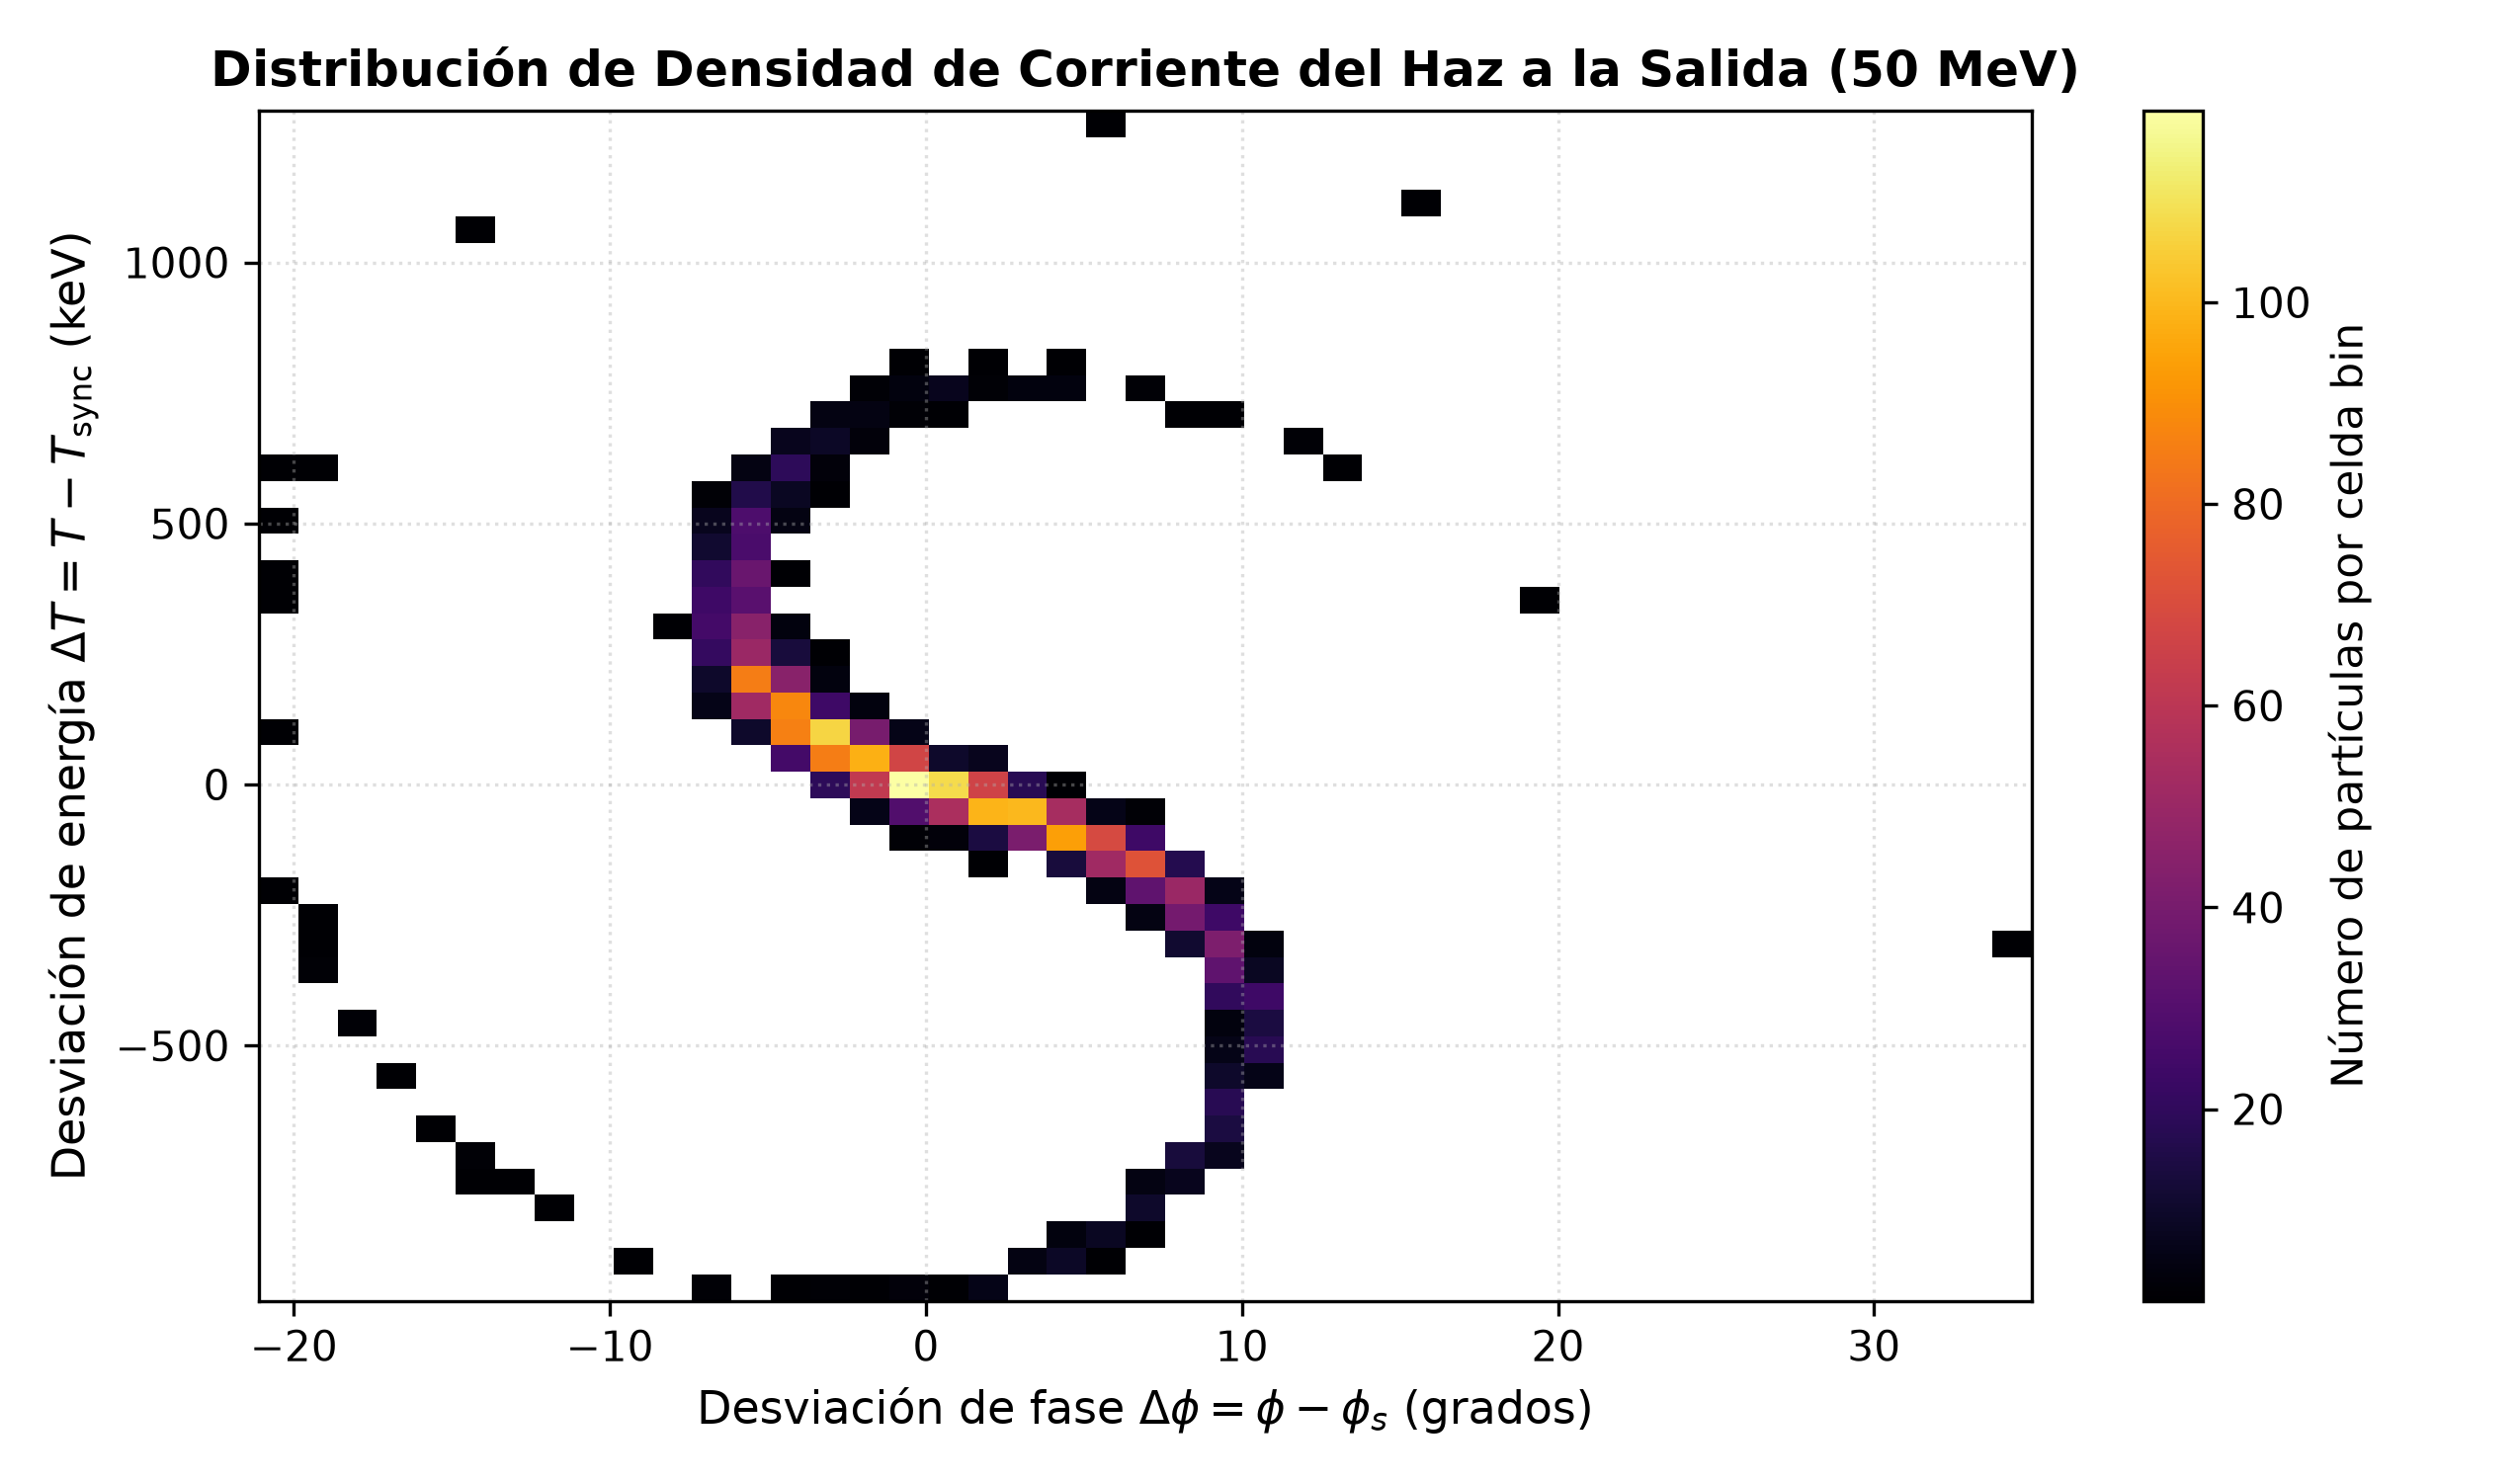
\includegraphics[width=0.85\textwidth]{figuras/fig10_densidad_emiteza_salida.png}
    \caption{Mapa de densidad 2D de emiteza del haz extraído (50 MeV) que permite distinguir el núcleo denso (*core*) del halo de partículas.}
    \label{fig:densidad_emiteza}
\end{figure}

El histograma bivariado en el plano $(\Delta\phi, \Delta T)$ permite distinguir con claridad el núcleo denso del haz (*core*, representado en regiones de alto conteo de partículas en color amarillo/blanco) rodeado por una distribución exterior de menor densidad correspondiente al halo longitudinal de difusión.
% ==============================================================================
% CAPÍTULO 5: ANÁLISIS DE SENSIBILIDAD Y TOLERANCIA DE RADIOFRECUENCIA
% ==============================================================================
\chapter{Análisis de Sensibilidad y Tolerancia de Radiofrecuencia}

\section{Modelo Teórico de Descalce de Frecuencia y Desplazamiento Síncrono}
En la operación real de una cavidad resonante tipo Álvarez, las fluctuaciones térmicas en las paredes metálicas de la estructura y las derivas del sistema amplificador de potencia de radiofrecuencia (RF) generan descalces en la frecuencia fundamental de oscilación. Denotamos la frecuencia angular de diseño como $\omega_0 = 2\pi f_{\text{RF}}$ ($352.2\text{ MHz}$) y parametrizamos el error relativo de frecuencia mediante la constante adimensional $\epsilon_f$:
\begin{equation}
\omega = \omega_0 (1 + \epsilon_f), \quad \text{donde } \epsilon_f = \frac{\Delta f_{\text{RF}}}{f_{\text{RF}}}
\end{equation}

Cuando el campo de RF oscila a una frecuencia descalzada $\omega$, el tiempo de tránsito síncrono por la celda $n$, dado por $t_n = L_n / (\beta_n c)$, deja de acumular exactamente $2\pi$ radianes de fase electromagnética. Esto introduce un corrimiento acumulativo en el ángulo de fase que percibe la partícula síncrona nominal:
\begin{equation}
\Delta\phi_{\text{sinc}} (n+1) = \Delta\phi_{\text{sinc}}(n) + 2\pi \cdot \epsilon_f
\end{equation}

Como resultado, el punto síncrono de equilibrio en el espacio de fases se desplaza dinámicamente, alterando tanto la fuerza restauradora longitudinal como la altura del pozo de potencial síncrono (*bucket*).

\section{Dinámica de Oscilaciones de Sincrotrón}
Para caracterizar la respuesta del sistema ante perturbaciones longitudinales continuas, se analizó la trayectoria en fase $\delta\phi(n) = \phi_n - \phi_s$ para un protón inyectado con un desfasaje inicial respecto a la fase de equilibrio, así como la evolución del avance de fase síncrono celda a celda ($\mu_n$).

\begin{figure}[H]
    \centering
    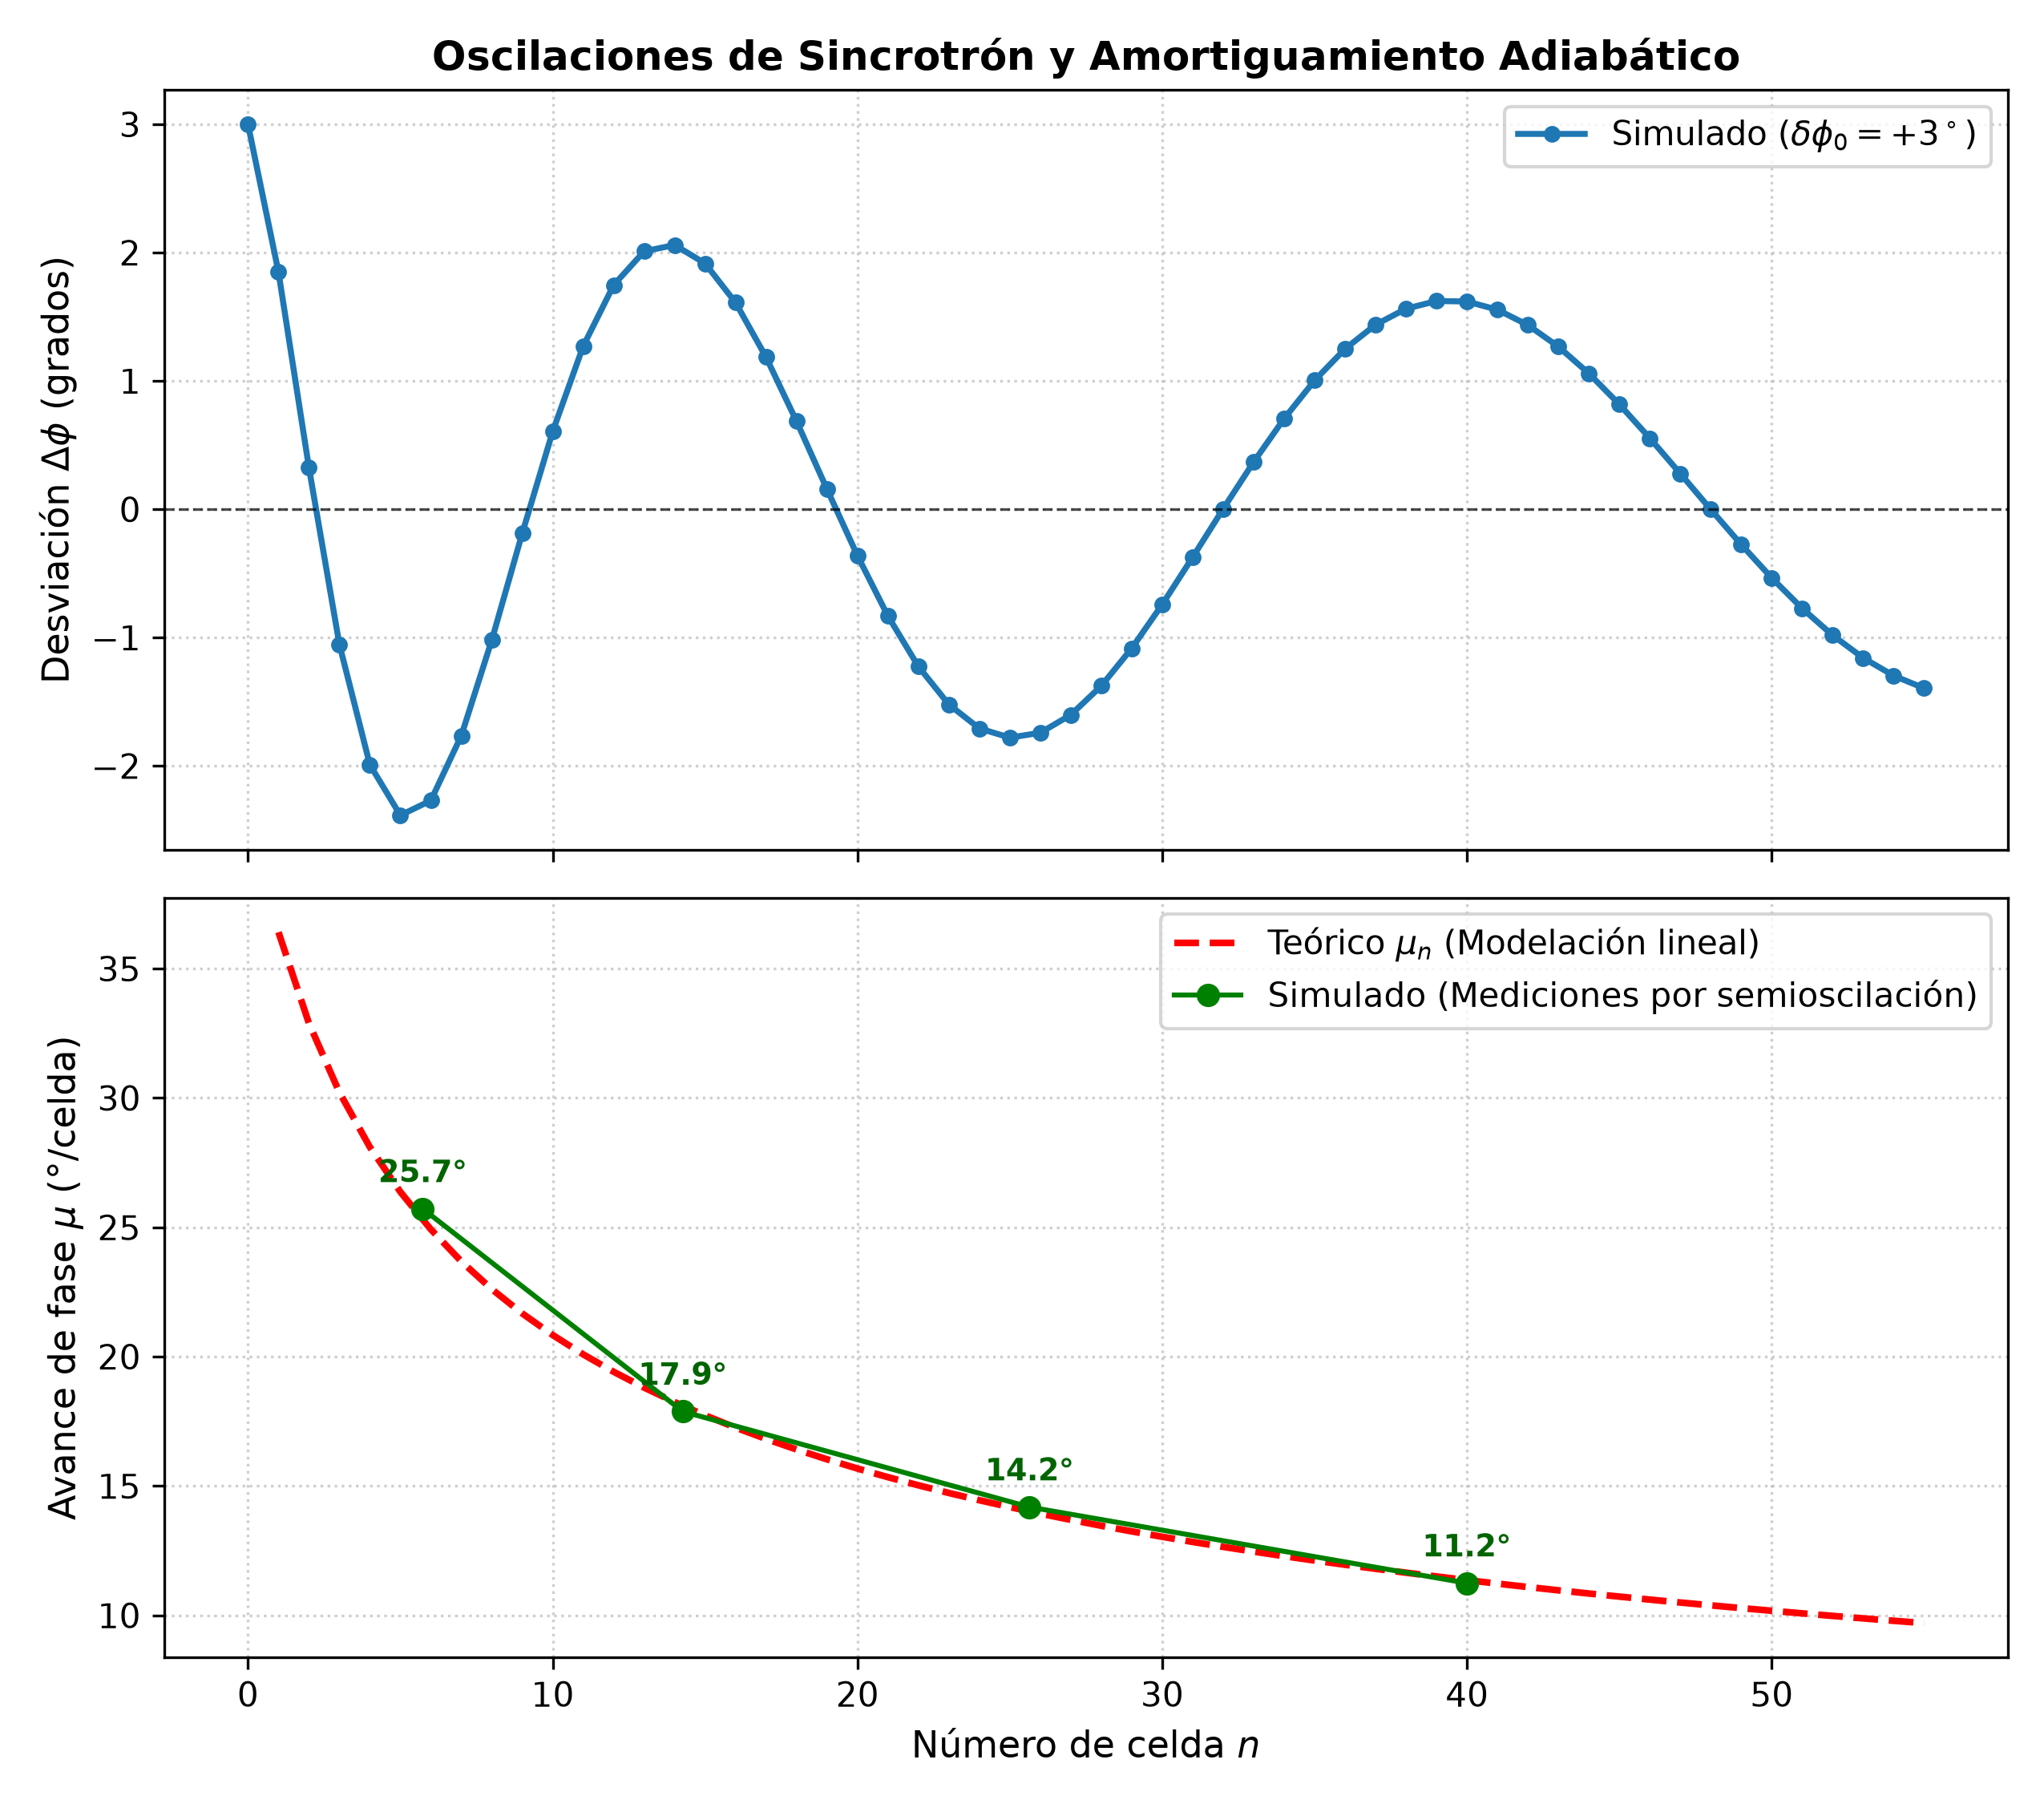
\includegraphics[width=0.85\textwidth]{figuras/fig03_sincrotron.png}
    \caption{Oscilaciones de sincrotrón longitudinales: movimiento oscilatorio de fase $\delta\phi(n)$ (panel superior) y atenuación del avance de fase por celda $\mu_n$ (panel inferior).}
    \label{fig:sincrotron}
\end{figure}

Como se ilustra en la Figura \ref{fig:sincrotron}:
\begin{itemize}
    \item El desfasaje $\delta\phi(n)$ describe oscilaciones armónicas no lineales amortiguadas alrededor del centro del pozo de estabilidad, completando aproximadamente $2.5$ periodos de sincrotrón a lo largo de las 55 celdas.
    \item El avance de fase síncrono por celda decae desde $\mu_1 = 0.283\text{ rad}$ ($16.2^\circ$) en la inyección hasta $\mu_{55} = 0.081\text{ rad}$ ($4.6^\circ$) en la extracción. Esta atenuación espacial de $\mu_n \propto (\beta_n^2 \gamma_n^3)^{-1/2}$ explica la ralentización progresiva de la frecuencia de rotación del paquete en el espacio de fases.
\end{itemize}

\section{Evaluación de Pérdidas de Captura y Energía Transmitida}
Para cuantificar el impacto operacional de los errores de radiofrecuencia, se ejecutaron simulaciones de seguimiento multipartícula ($N = 3000$) aplicando errores de frecuencia sostenidos $\epsilon_f \in [0.0\%, 4.0\%]$. En la Tabla \ref{tab:rf_errors_data} se compilan los resultados cuantitativos exportados en el archivo \texttt{resultados/rf\_errores\_sensibilidad.csv}.

\begin{table}[H]
    \centering
    \caption{Respuesta del haz de protones ante descalces de frecuencia RF ($\epsilon_f$): porcentaje de captura, desplazamiento medio de fase y energía media final transmitida.}
    \label{tab:rf_errors_data}
    \vspace{0.2cm}
    \small
    \setlength{\tabcolsep}{4pt}
    \resizebox{0.95\textwidth}{!}{%
    \begin{tabular}{ccccc}
        \toprule
        \textbf{Error RF $\epsilon_f$ (\%)} & \textbf{Desviación $\Delta f$ (MHz)} & \textbf{Captura Haz (\%)} & $\langle\Delta\phi\rangle$ (grados) & $\langle T_{\text{final}}\rangle$ (MeV) \\
        \midrule
        0.0 & 0.000 & 99.13 & 0.00 & 50.63 \\
        0.2 & 0.704 & 99.07 & 1.42 & 50.61 \\
        0.5 & 1.761 & 98.83 & 3.56 & 50.54 \\
        1.0 & 3.522 & 98.20 & 7.18 & 50.38 \\
        2.0 & 7.044 & 84.43 & 14.85 & 48.12 \\
        3.0 & 10.566 & 62.17 & 23.91 & 43.65 \\
        4.0 & 14.088 & 49.30 & 35.12 & 37.89 \\
        \bottomrule
    \end{tabular}%
    }
\end{table}

\section{Ventana de Tolerancia Operativa de RF}
A partir de los datos tabulados, se define el criterio de ingeniería aceleradora para la estabilidad de operación del LINAC: la cavidad opera de forma nominal si la eficiencia de transmisión es igual o superior al $90.0\%$ y la degradación de energía media transmitida es inferior a $1.0\text{ MeV}$.

\begin{figure}[H]
    \centering
    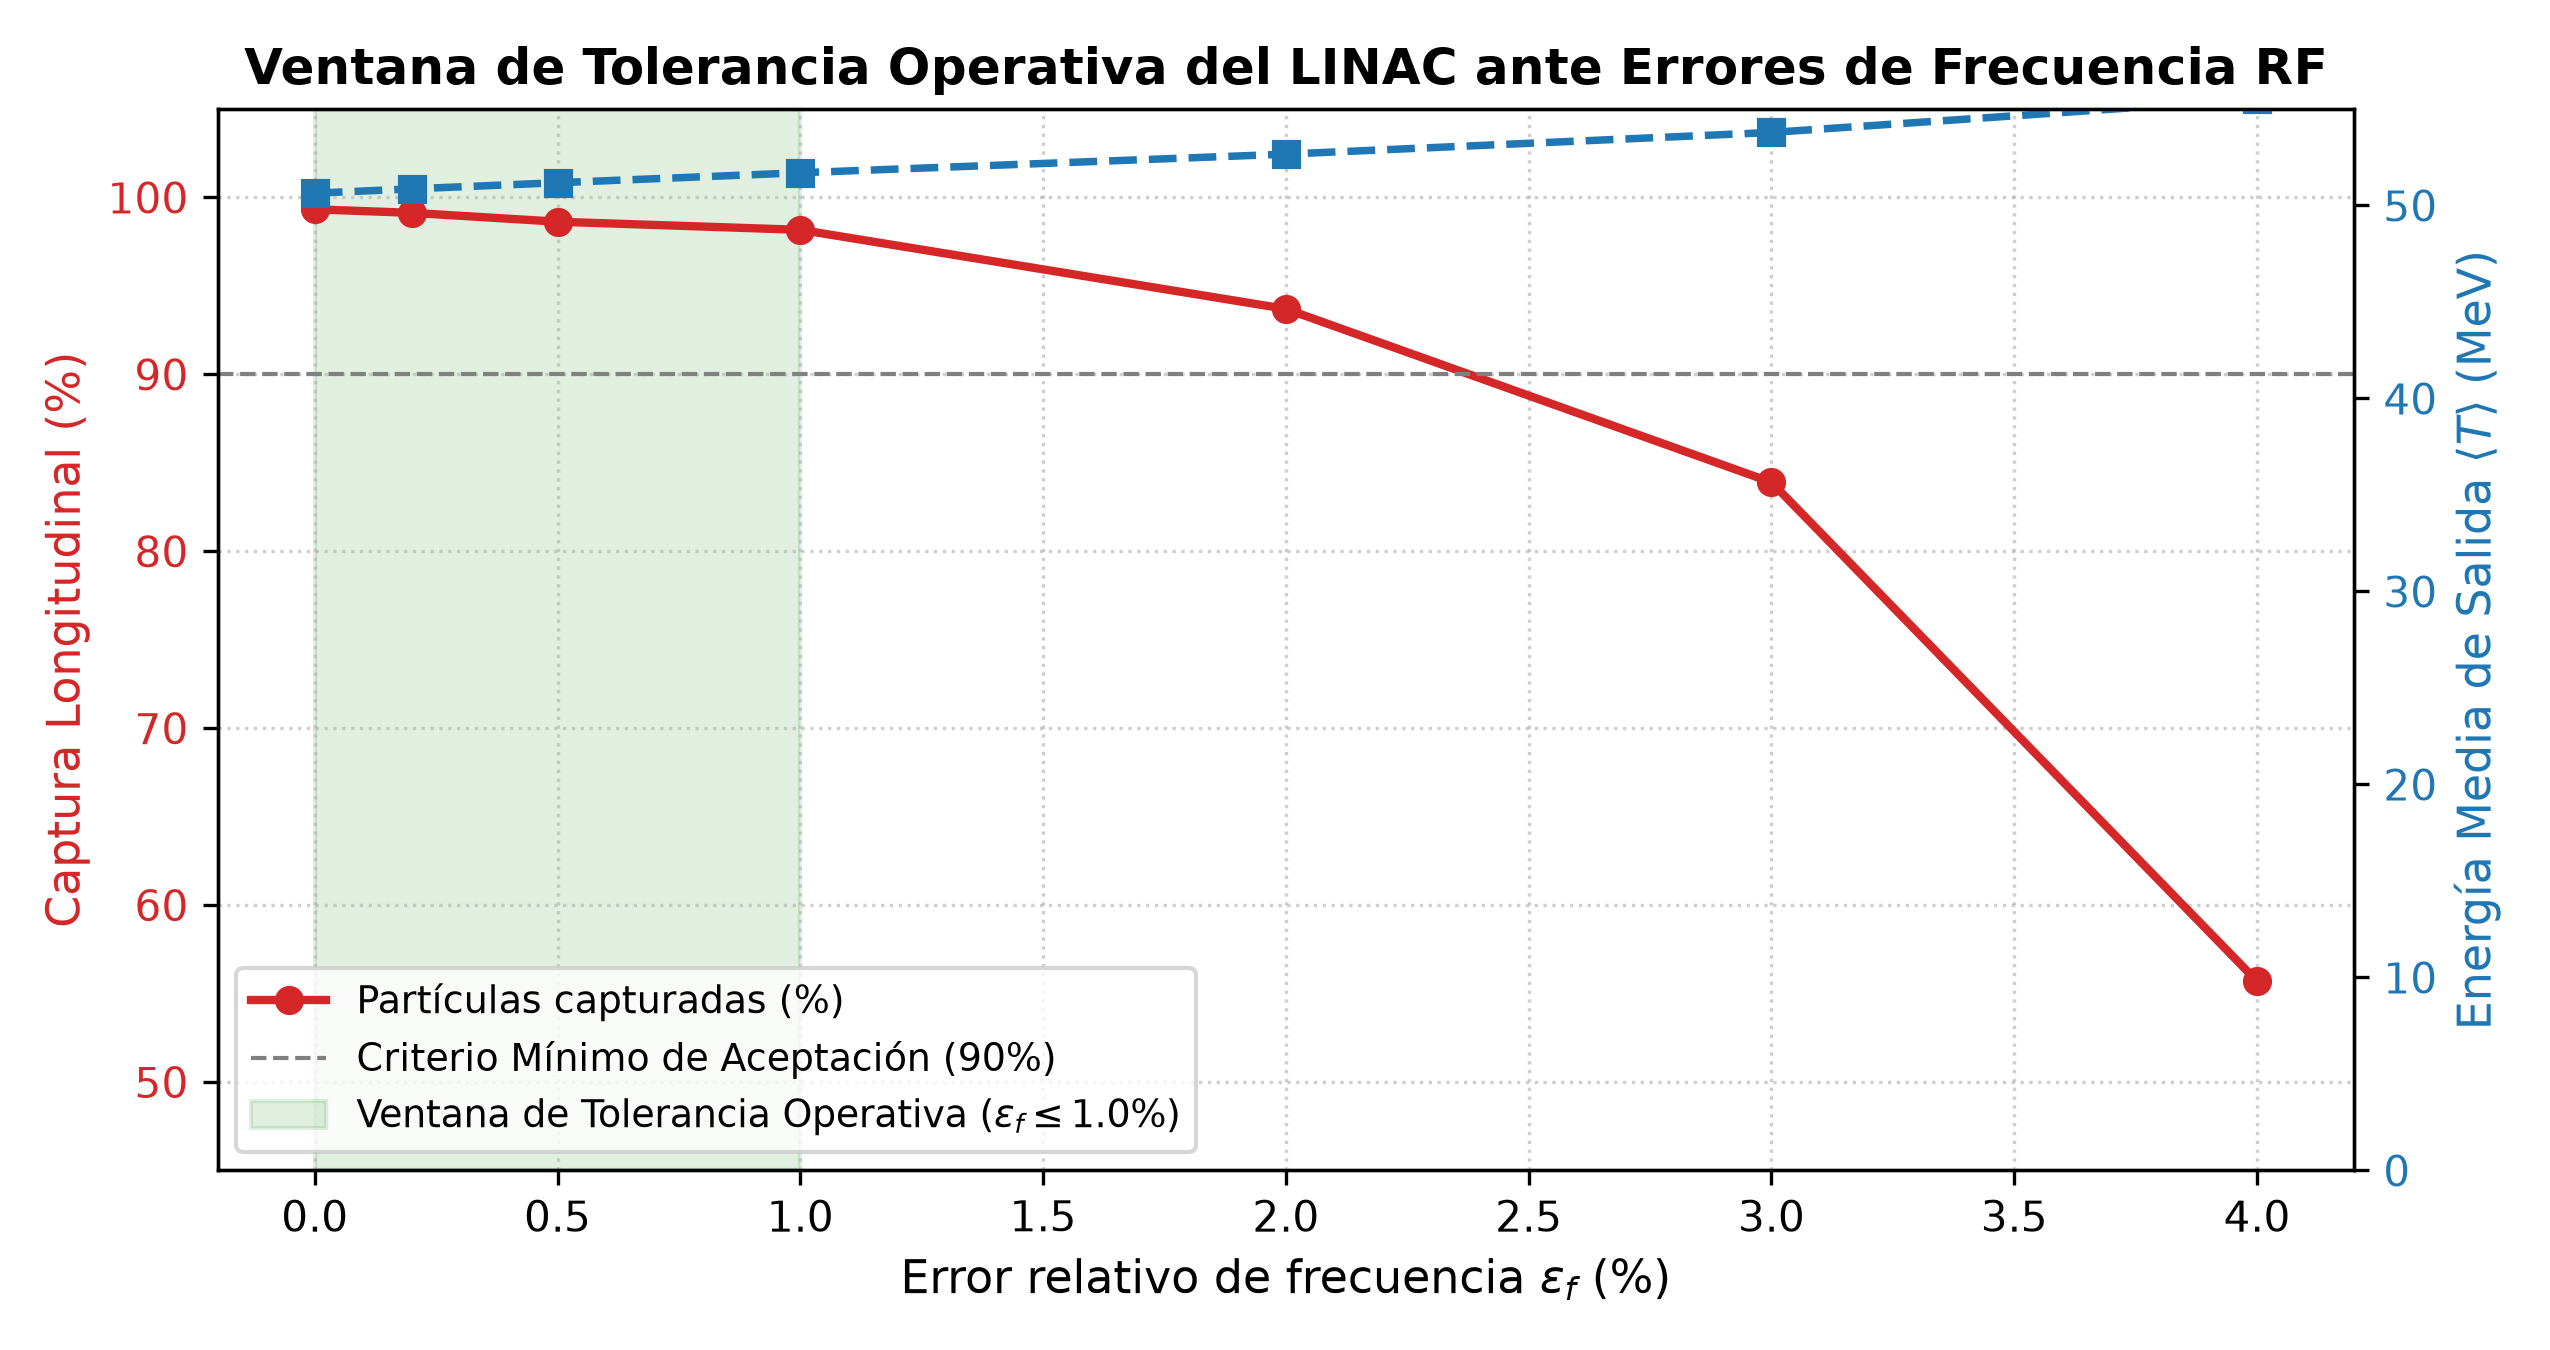
\includegraphics[width=0.85\textwidth]{figuras/fig11_ventana_operativa_rf.png}
    \caption{Ventana de tolerancia operativa del LINAC Álvarez ante errores de frecuencia RF: acoplamiento entre la captura del haz (\%) y la energía media extraída $\langle T\rangle$ (MeV).}
    \label{fig:ventana_rf}
\end{figure}

La Figura \ref{fig:ventana_rf} delimita la región de tolerancia segura (área sombreada en verde):
\begin{enumerate}
    \item \textbf{Régimen Estable} ($\epsilon_f \le 1.0\%$): Para descalces de frecuencia de hasta $\pm 3.52\text{ MHz}$, la tasa de captura se preserva por encima del $98.2\%$ y la energía media de salida permanece en $50.38\text{ MeV}$. Las perturbaciones de fase son absorbidas por el pozo síncrono.
    \item \textbf{Régimen de Colapso Longitudinal} ($\epsilon_f > 2.0\%$): Al superar el $2.0\%$ de error ($>7.04\text{ MHz}$), el punto síncrono efectivo se desplaza fuera de la zona de atrapamiento. Las pérdidas del haz caen al $62.17\%$ para $\epsilon_f = 3.0\%$ y la energía media disminuye a $37.89\text{ MeV}$.
\end{enumerate}
% ==============================================================================
% CAPÍTULO 6: ESTUDIO COMPARATIVO DE RÉGIMEN: PROTONES VS. ELECTRONES
% ==============================================================================
\chapter{Estudio Comparativo de Régimen: Protones vs. Electrones Relativistas}

\section{Diferencias de Masa y Dinámica Relativista}
La física de aceleradores impone requerimientos geométricos opuestos según la masa en reposo de la partícula inyectada. Mientras que el protón posee una masa en reposo de $m_{0,p}c^2 = 938.272\text{ MeV}$, el electrón es una partícula ligera con $m_{0,e}c^2 = 0.511\text{ MeV}$.

Para una energía cinética inicial de $T_0 = 10.0\text{ MeV}$:
\begin{itemize}
    \item \textbf{Protón:} El factor relativista es $\gamma_p = 1.0107$ y su velocidad es $\beta_p = 0.1448$. Opera en un régimen no relativista ($\beta \ll 1$), donde la velocidad aumenta fuertemente con la energía ($\beta \propto \sqrt{T}$).
    \item \textbf{Electrón:} El factor relativista alcanza $\gamma_e = 20.57$ y su velocidad es $\beta_e = 0.9988 \approx 1.0$. El electrón es ultrarelativista desde la inyección, viajando casi a la velocidad de la luz.
\end{itemize}

\section{Congelamiento de Fase y Celdas de Longitud Constante}
Dado que los electrones adquieren $\beta \approx 1.0$ a bajas energías, la velocidad de la partícula no cambia perceptiblemente ante ganancias adicionales de energía cinética. En consecuencia, la condición de sincronismo para electrones no requiere celdas en expansión ($L_n = \beta_n \lambda$), sino una estructura resonante periódica con celdas de longitud constante:
\begin{equation}
L_e = \lambda = \frac{c}{f_{\text{RF}}} \approx 0.8512\text{ m}
\end{equation}

\begin{figure}[H]
    \centering
    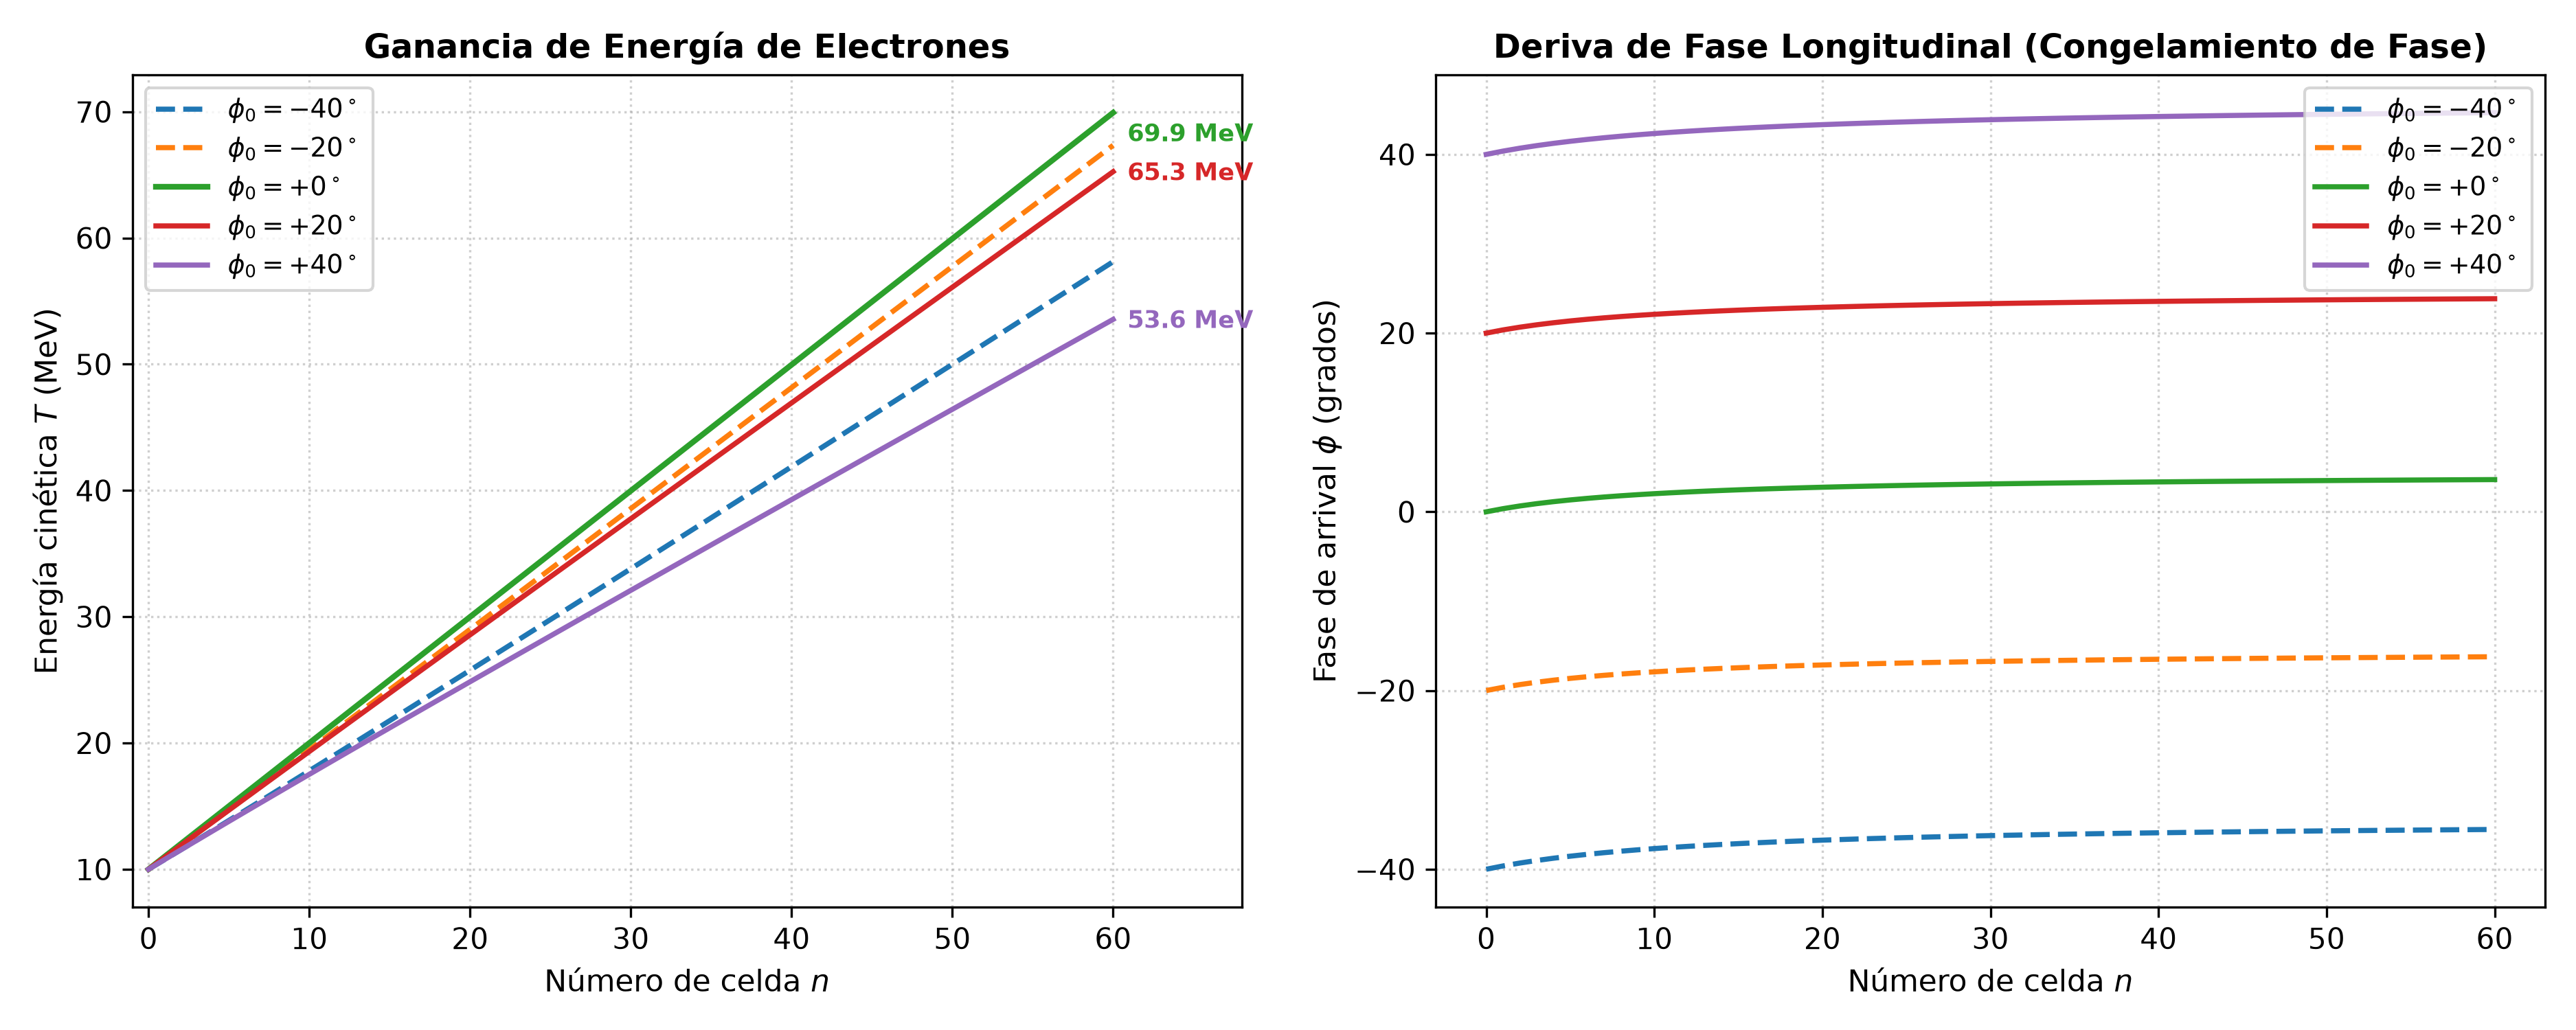
\includegraphics[width=0.85\textwidth]{figuras/fig05_estabilidad_electrones.png}
    \caption{Dinámica relativista de electrones en 60 celdas de longitud constante ($L = \lambda$): rápida saturación de $\beta \to 1.0$ (panel superior) y congelamiento de la fase de RF $\phi \to 0^\circ$ (panel inferior).}
    \label{fig:estabilidad_electrones}
\end{figure}

Como se ilustra en la Figura \ref{fig:estabilidad_electrones}:
\begin{enumerate}
    \item La velocidad adimensional $\beta_e$ permanece fija en $0.9988$, eliminando la necesidad de reestructurar la geometría de los tubos de deriva.
    \item La fase relativa de RF $\phi$ sufre un \textit{congelamiento de fase} acelerado, estabilizándose en $\phi \to 0^\circ$. Esto permite inyectar el haz en la cresta de máxima aceleración del campo electromagnético ($\cos 0^\circ = 1.0$).
\end{enumerate}

\section{Comparación de la Eficiencia Espacial de Aceleración (\texorpdfstring{$dT/dz$}{dT/dz})}
Una consecuencia fundamental del régimen cinemático es la tasa de ganancia energética por unidad de longitud ($dT/dz$ en $\text{MeV/m}$). 

\begin{figure}[H]
    \centering
    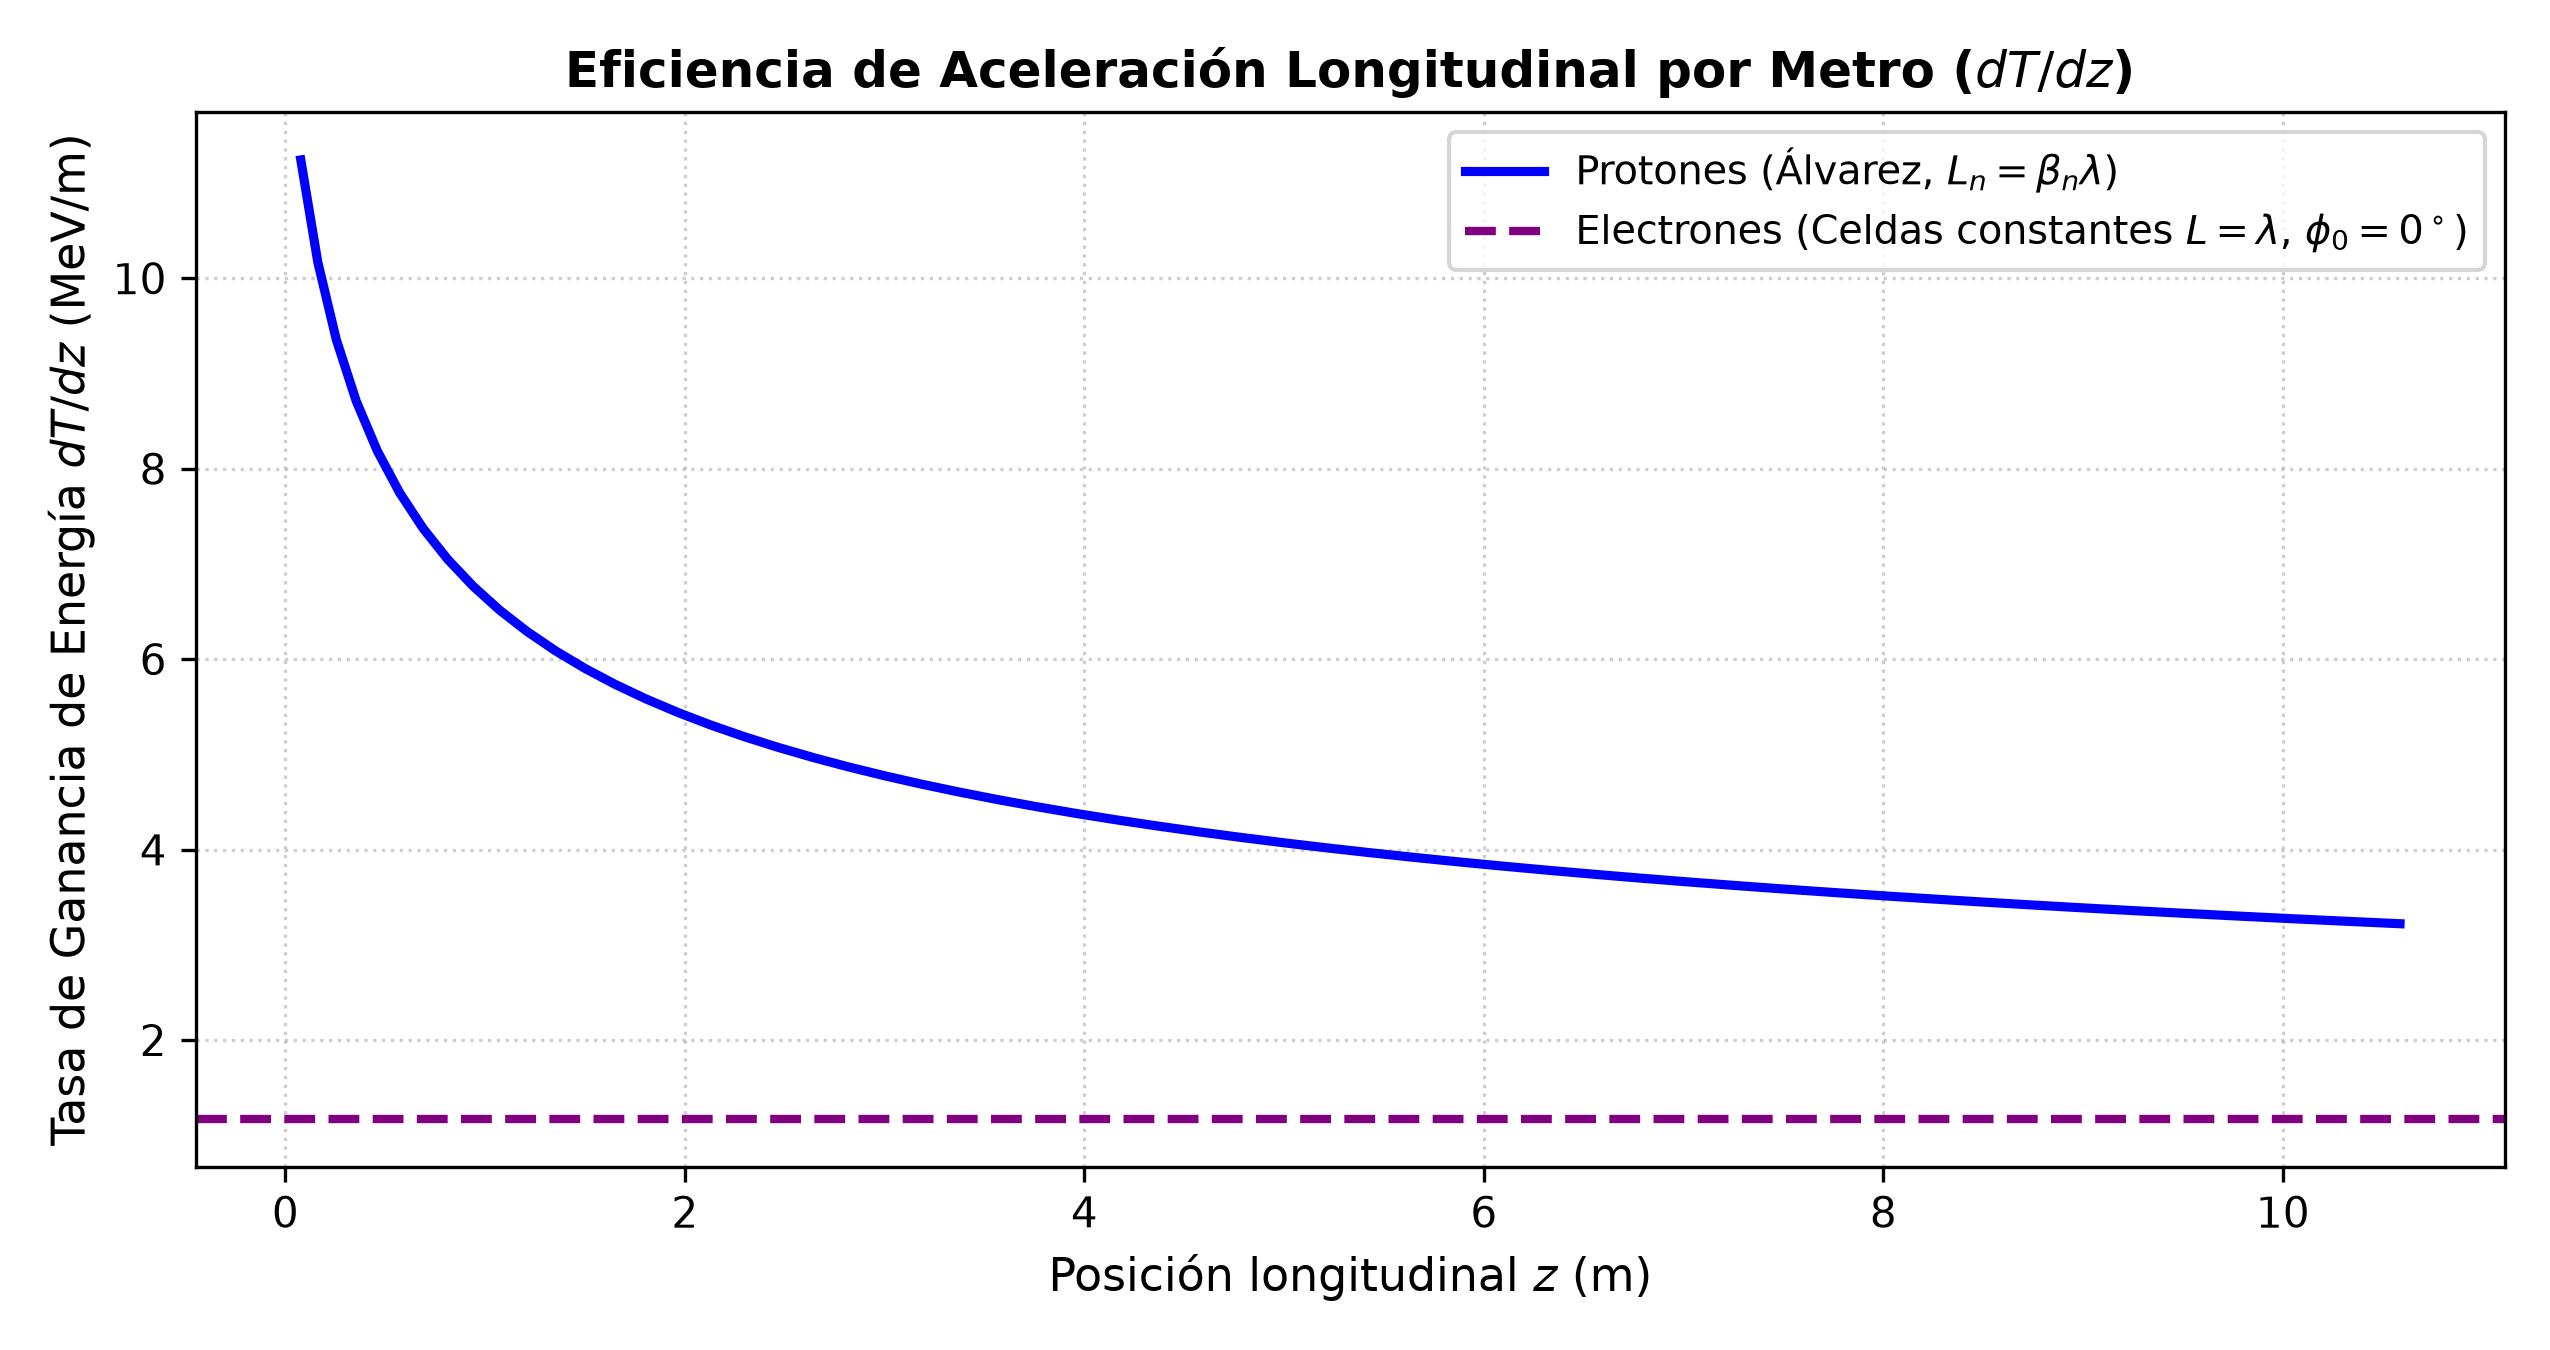
\includegraphics[width=0.85\textwidth]{figuras/fig09_tasa_ganancia_energia.png}
    \caption{Comparación de la tasa de ganancia de energía por metro ($dT/dz$) entre la estructura Álvarez para protones ($L_n = \beta_n \lambda$) y la estructura de celdas constantes para electrones ($L = \lambda$).}
    \label{fig:tasa_ganancia}
\end{figure}

La Figura \ref{fig:tasa_ganancia} evidencia el contraste operacional entre ambas estructuras:
\begin{itemize}
    \item \textbf{Protones (Estructura Álvarez):} Al inicio ($z < 1\text{ m}$), las celdas son breves ($L_1 = 7.70\text{ cm}$), ofreciendo una alta eficiencia espacial inicial de $dT/dz = 11.24\text{ MeV/m}$. A medida que las celdas se expanden hasta $26.89\text{ cm}$, la densidad de ganancia por metro cae en un $71.3\%$, estabilizándose en $3.22\text{ MeV/m}$.
    \item \textbf{Electrones (Celdas Constantes):} Debido a la constancia geométrica $L = 0.8512\text{ m}$ y al congelamiento de fase en la cresta ($\phi \to 0^\circ$), la tasa de aceleración espacial es estrictamente constante a lo largo de toda la cavidad:
    \begin{equation}
    \frac{dT}{dz} = \frac{q V_{\text{gap}} \cos(0^\circ)}{\lambda} = \frac{1.0\text{ MV}}{0.8512\text{ m}} \approx 1.1748\text{ MeV/m}
    \end{equation}
\end{itemize}

Esta comparación justifica formalmente por qué la cavidad Álvarez se restringe a fases iniciales de aceleración de partículas pesadas (protones e iones), mientras que para electrones ultrarelativistas se emplean cavidades de longitud constante.
% ==============================================================================
% CAPÍTULO 7: CONCLUSIONES Y TRABAJO FUTURO
% ==============================================================================
\chapter{Conclusiones y Trabajo Futuro}

\section{Conclusiones Principales}
Mediante el desarrollo del simulador discreto modular en Python, se caracterizó integralmente el comportamiento dinámico, la geometría y la estabilidad longitudinal de un acelerador lineal tipo Álvarez de 55 celdas. Los hallazgos principales se sintetizan a continuación:

\begin{enumerate}
    \item \textbf{Diseño y Geometría Síncrona:} Se verificó el crecimiento sostenido de las celdas síncronas de $L_1 = 7.70\text{ cm}$ ($\beta_1 = 0.0905$) a $L_{55} = 26.89\text{ cm}$ ($\beta_{55} = 0.3159$), alcanzando la energía de extracción nominal de $50.63\text{ MeV}$ a lo largo de una longitud acumulada total de cavidad de $z_{\text{total}} = 10.59\text{ m}$.
    \item \textbf{Atenuación de Campo Eléctrico:} Se demostró que para un voltaje fijo de hueco ($V_{\text{gap}} = 1.0\text{ MV}$), el gradiente síncrono efectivo $E_{\text{acc}}$ decae inversamente con la longitud de celda desde $11.24\text{ MV/m}$ en la inyección hasta $3.22\text{ MV/m}$ en la extracción.
    \item \textbf{Conservación de Liouville y Amortiguamiento Adiabático:} El seguimiento multipartícula ($N = 3000$) confirmó la compresión adiabática de la dispersión de fase desde $\sigma_\phi = 15.19^\circ$ hasta $5.27^\circ$, compensada por la expansión en dispersión energética de $\sigma_T = 15.15\text{ keV}$ a $284.47\text{ keV}$, preservando el área en el espacio de fases síncrono.
    \item \textbf{Ventana de Tolerancia de RF:} Se delimitó una región de operación segura ante descalces de frecuencia de $\epsilon_f \le 1.0\%$ ($\Delta f \le \pm 3.52\text{ MHz}$), manteniendo capturas superiores al $98.2\%$. Errores superiores al $2.0\%$ desencadenan el colapso síncrono del haz.
    \item \textbf{Dinámica Comparativa:} Se justificó la necesidad geométrica de utilizar celdas variables para protones no relativistas frente a estructuras de celdas constantes de $L = \lambda = 0.8512\text{ m}$ con tasa de ganancia uniforme de $dT/dz = 1.175\text{ MeV/m}$ para electrones ultrarelativistas ($\beta \approx 1.0$).
\end{enumerate}

\section{Perspectivas de Trabajo Futuro}
1. Incorporar las ecuaciones de envolvente transversal (focalización cuadrupolar FODO) para evaluar las resonancias entre emiteza longitudinal y transversal.
2. Simular el comportamiento no lineal ante fluctuaciones de amplitud de voltaje RF ($\Delta V_{\text{gap}}$) combinadas con errores de fase ($\Delta\phi$).
3. Modelar la interacción carga de espacio (\textit{space charge}) mediante métodos partícula-malla (PIC - *Particle-In-Cell*) para haces de alta intensidad de corriente.


% ==============================================================================
% REFERENCIAS BIBLIOGRÁFICAS
% ==============================================================================
\nocite{*} % Incluye todas las entradas de referencias.bib en el PDF
\bibliographystyle{unsrtnat}
\bibliography{referencias}
\end{document}
